\setchapterstyle{kao}
\chapter{Three-flavor oscillation measurement}
\setchapterpreamble[u]{\margintoc}
\labch{measurement-three-flavor}

The first measurement made using the data sample described in this work is the measurement of the atmospheric mixing angle $\theta_{23}$ and the mass splitting $\Delta m^2_{32}$. The experimental setup of DeepCore is ideally suited for this measurement, because the first valley of maximum disappearance for muon neutrinos passing through the entire diameter of the Earth is expected to lie between 20~GeV and 30~GeV as shown in \reffig{three-flavor-oscprob} in \refsec{atmospheric-neutrino-oscillations}. The parameter $\Delta m^2_{32}$ changes the position of the oscillation valley, while $\theta_{23}$ changes its depth. In the analysis histogram, this disappearance effect is evident even with the eye alone in the PID channel for highly track-like events, as shown in \reffig{nominal-hist-null-hypo}. For this measurement, oscillation probabilities are calculated in the three-flavor oscillation scheme including matter effects. The matter profile of Earth is modeled as a shells of constant density following the Preliminary Reference Earth Model (PREM)\sidecite{PREM}. The Monte-Carlo simulated events are weighted in a staged procedure where each stage updates the event weights according to flux, cross-sections and oscillation probabilities\sidecite{PISA}. The oscillation probabilities are calculated using a \textsc{Python} implementation of the Barger~et~al.\sidecite{barger-oscillations} calculation.

%\begin{figure}
%    \centering
%    %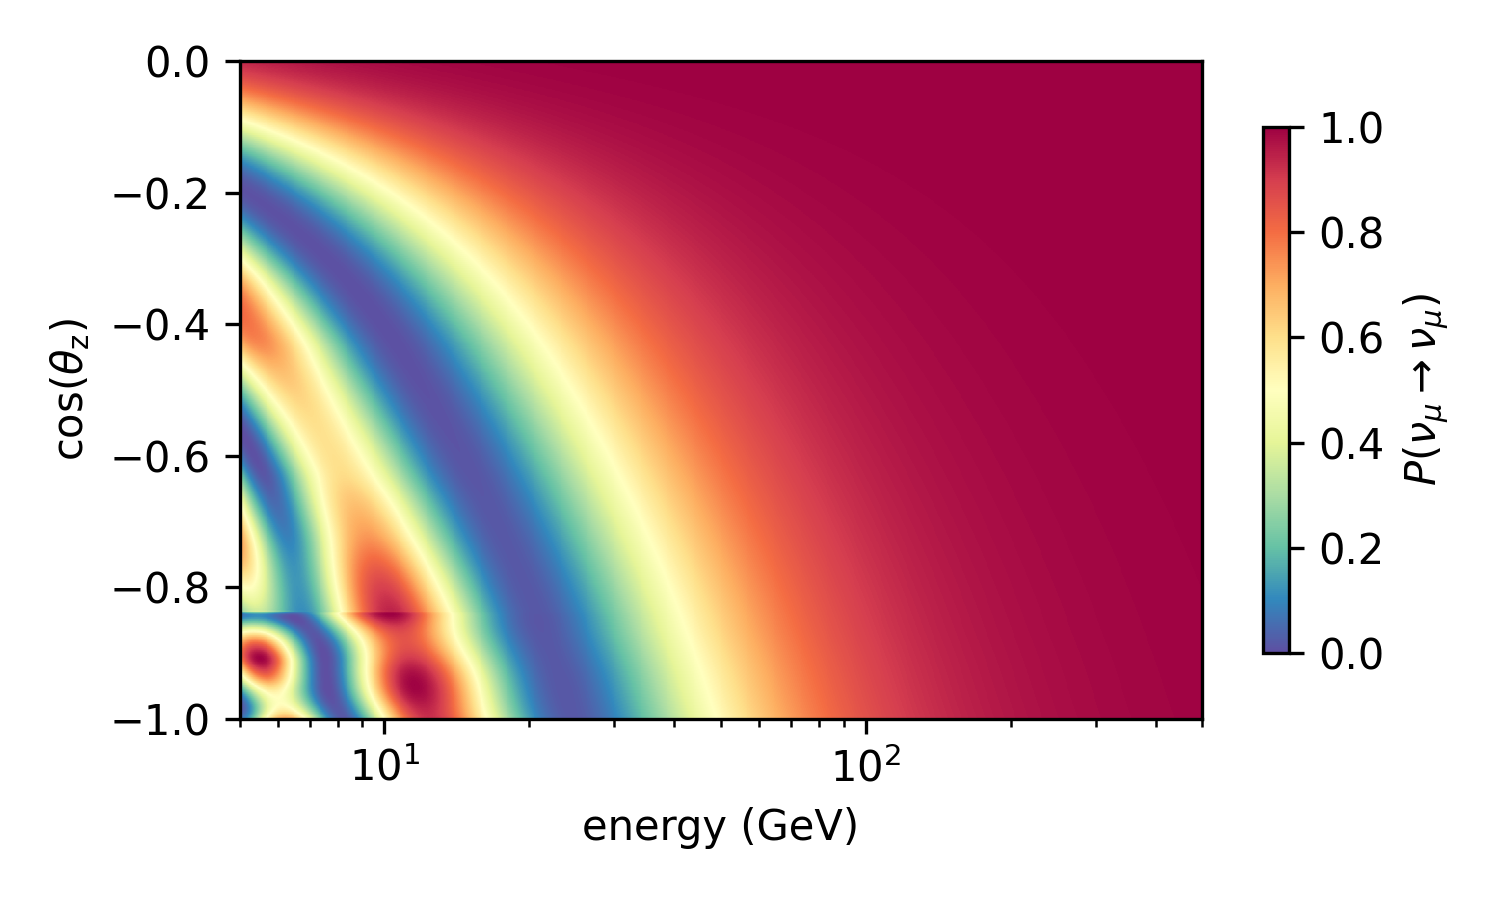
\includegraphics[width=0.9\linewidth]{figures/measurement/three_flavor/numu_surv_prob_no_sterile_no_text.png}
%    \tikzsetnextfilename{numu_surv_prob_no_sterile}%
\begin{tikzpicture}

\definecolor{darkgray176}{RGB}{176,176,176}

\begin{axis}[
    % it is important to set this option only for the axis, not for the entire plot!
    % Otherwise, the label of the colorbar will be cut off... 
    set layers=axis on top,
    colorbar,
    colorbar style={
        ylabel={$P(\nu_\mu\rightarrow\nu_\mu)$},
        tick pos=right,
        ytick style={color=black},
        tick align=outside
    },
    colormap={mymap}{[1pt]
      rgb(0pt)=(0.368627450980392,0.309803921568627,0.635294117647059);
      rgb(1pt)=(0.196078431372549,0.533333333333333,0.741176470588235);
      rgb(2pt)=(0.4,0.76078431372549,0.647058823529412);
      rgb(3pt)=(0.670588235294118,0.866666666666667,0.643137254901961);
      rgb(4pt)=(0.901960784313726,0.96078431372549,0.596078431372549);
      rgb(5pt)=(1,1,0.749019607843137);
      rgb(6pt)=(0.996078431372549,0.87843137254902,0.545098039215686);
      rgb(7pt)=(0.992156862745098,0.682352941176471,0.380392156862745);
      rgb(8pt)=(0.956862745098039,0.427450980392157,0.262745098039216);
      rgb(9pt)=(0.835294117647059,0.243137254901961,0.309803921568627);
      rgb(10pt)=(0.619607843137255,0.00392156862745098,0.258823529411765)
    },
    log basis x={10},
    point meta max=1,
    point meta min=0,
    tick align=outside,
    tick pos=left,
    x grid style={darkgray176},
    xlabel={energy (GeV)},
    xmin=5, xmax=500,
    xmode=log,
    xtick style={color=black},
    y grid style={darkgray176},
    ylabel={\(\displaystyle \cos(\theta_{\mathrm{z}})\)},
    ymin=-1, ymax=0,
    ytick style={color=black}
]
\addplot graphics [includegraphics cmd=\pgfimage,xmin=5, xmax=500, ymin=-1, ymax=0] {figures/measurement/three_flavor/oscillograms/numu_surv_prob_no_sterile-000.png};
\end{axis}

\end{tikzpicture}

%    \caption{Muon-neutrino survival probability calculated at \textsc{NuFit~4.0}\cite{nufit40} global best fit parameters.}
%    \label{fig:three-flavor-oscprob}
%\end{figure}

\section{Statistical Analysis}

\subsection{Definition of test statistic}
\label{sec:test-statistic}

To make a measurement, the discrepancy between the histograms of the reweighted MC events and the observed data events has to be measured by an appropriate test statistic. This measurement uses a modified $\chi^2$ test statistic defined as
\begin{equation}
\chi^2_{\mathrm{mod}} = \sum_{i \in \mathrm{bins}}^{}\frac{(N^{\nu}_i + N^{\mu}_i - N^{\mathrm{obs}}_i)^2}{N^{\nu}_i + N^{\mu}_i + (\sigma^{\nu}_i)^2 + (\sigma^{\mu}_i)^2} + \sum_{j \in \mathrm{syst}}^{}\frac{(s_j - \hat{s_j})^2}{\sigma^2_{s_j}},
\label{eq:mod-chi2}
\end{equation}
\noindent where $N^{\nu}_i$ and $N^{\mu}_i$ are the expectation values for neutrinos and atmospheric muons, respectively, and $N^{\mathrm{obs}}_i$ is the number of observed events. The expectation value for neutrinos within a bin is calculated as the sum of the neutrino MC event weights $N^{\nu}_i = \sum_{i}^{\nu\,\mathrm{evts}} w_i$, with the statistical uncertainty due to finite simulation statistics $(\sigma^{\nu}_i)^2 = \sum_{i}^{\mathrm{evts}} w_i^2$. The expectation value for muons, $N^{\mu}_i$, is taken from the KDE-smoothed template shown in \reffig{muon-kde-smoothing}. The variance of the KDE estimate, $(\sigma^{\mu}_i)^2$, is calculated from a heuristic described below. The error term due to Poisson fluctuations of the data is calculated with the total MC expectation for muons and neutrinos. The second term in equation~\ref{eq:mod-chi2} is included as a penalty term to account for prior knowledge of some systematic parameters. 

\subsubsection{Muon KDE error estimates}
For the three-flavor oscillation analysis, the variance of the muon KDE estimate is calculated using a heuristic based on the theoretical upper bound of the variance of a KDE estimate with a fixed kernel. If the KDE estimate of the density at the point $x_0$ given $n$ i.i.d. samples from the true PDF $p$ is $\hat{p}_n(x_0)$, the upper bound on the variance is
\begin{equation}
    \mathrm{Var}(\hat{p}_n(x_0)) \leq \frac{1}{nh}p(x_0)\sigma_K^2\;,\label{eq:kde-var-upper-bound}
\end{equation}
where $h$ is the bandwidth and $\sigma_K^2=\int K^2(y)\,\mathrm{d}y$ with $K$ being the kernel function. The true PDF can be approximated with the estimated PDF to obtain an approximate error estimate. However, the KDE implementation used in this analysis uses a dynamic bandwidth and does not readily give access to $\sigma_K^2$ either. For this reason, an ad hoc heuristic is used following
\begin{equation}
    (\sigma^{\mu}_i)^2 = \mathrm{Var}(\hat{p}_n(x_0))\approx C\frac{\hat{p}_n(x_0)}{n}\;,\label{eq:kde-var-ad-hoc}
\end{equation}
where $C$ is an overall scaling factor that has to be tuned ''by hand''. To do this, a least-squares fit is run on the systematic MC sets and the value of $C$ is chosen such that the average $\chi^2/\mathrm{dof}$ from the least-squares fits over all bins is $\approx 1$ when $n$ is the number \emph{unweighted} events in the muon MC sample. This heuristic encodes the fact that the variance of the KDE estimate should be proportional to the density and inversely proportional to the number of MC events, where the proportionality factor is tuned to the statistical fluctuations between independent MC sets.

\subsection{Modeling of Detector Response}
\label{sec:hypersurfaces}

\begin{marginfigure}[\baselineskip]
    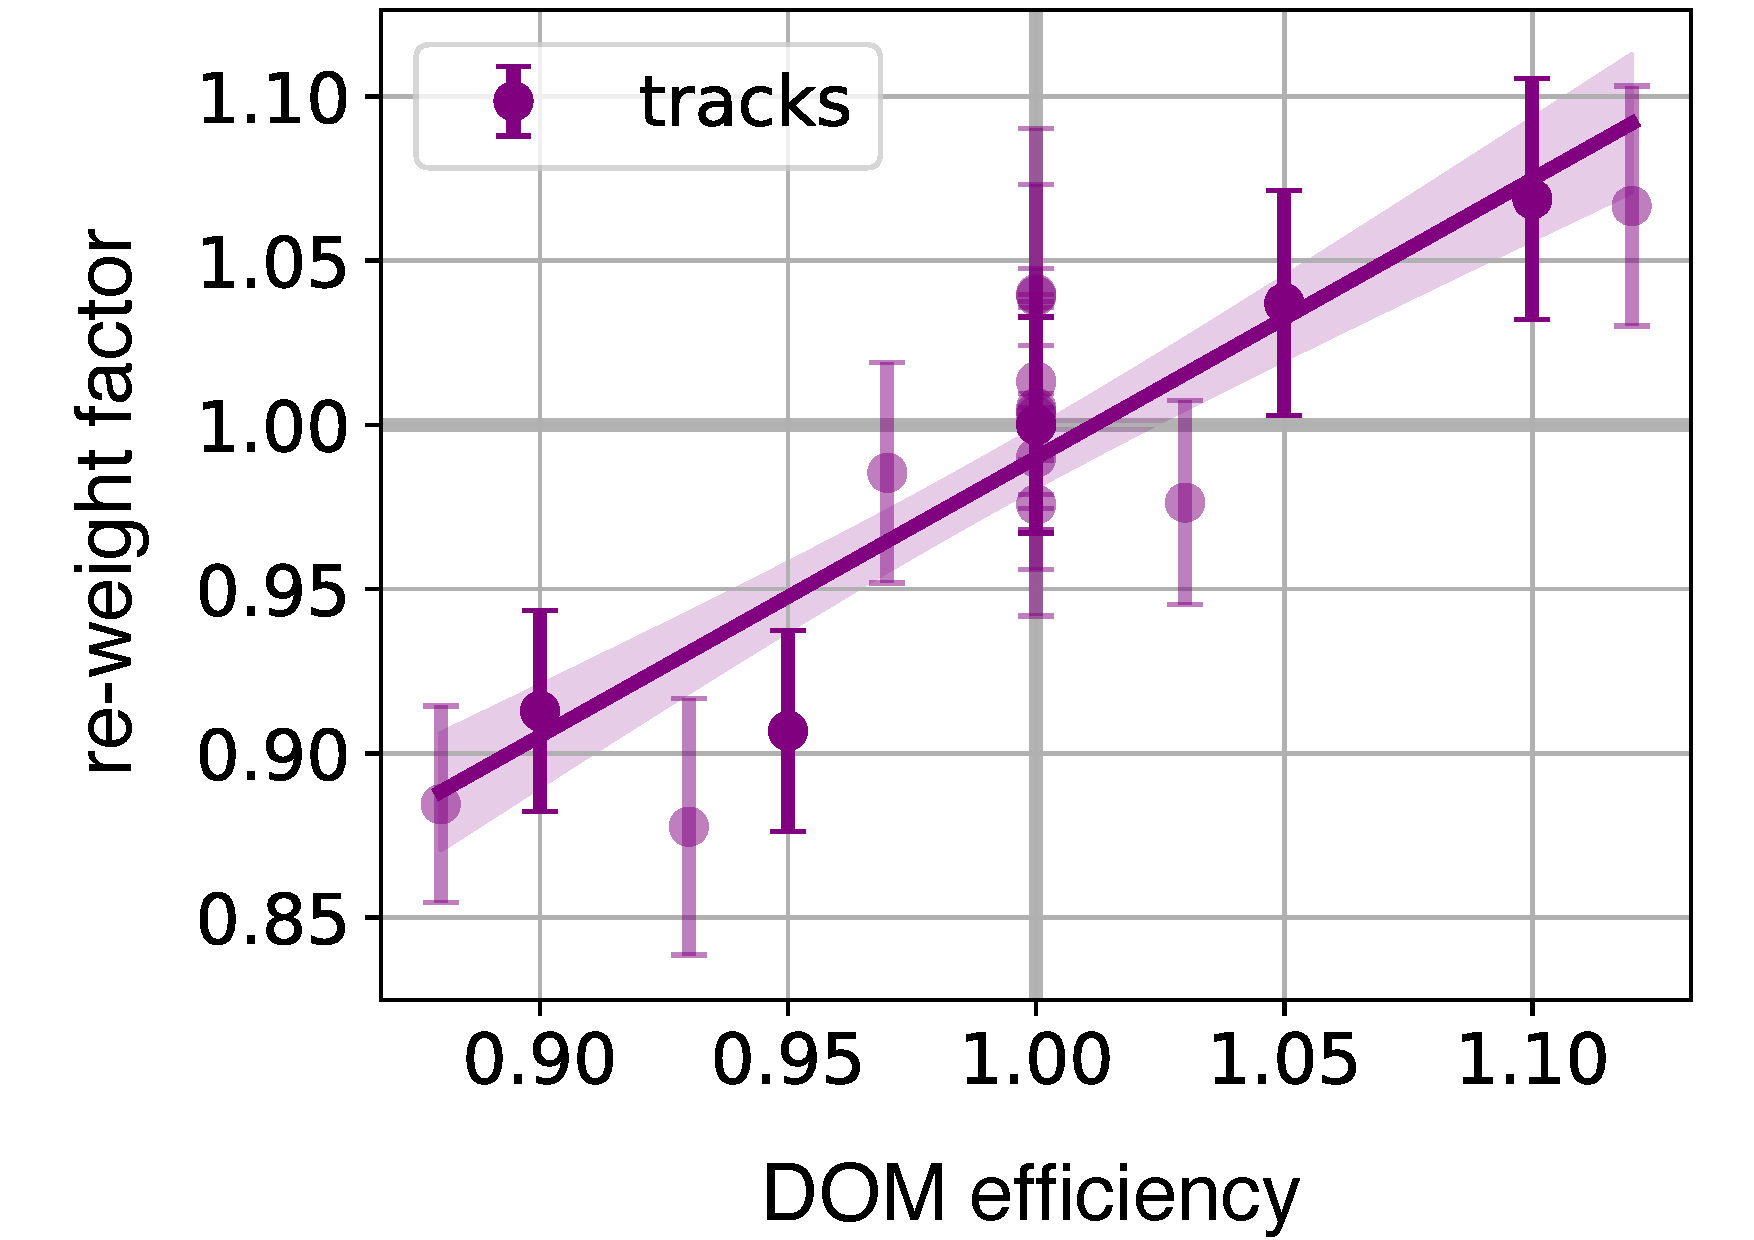
\includegraphics[width=\linewidth]{figures/measurement/systematics/detector/hypersurface_example_v2.pdf} 
    \caption{Example of a linear regression in one bin of the analysis projected onto the dimension of the DOM efficiency. Data points with translucent error bars originate from MC sets where one or more parameters besides DOM efficiency are at off-nominal points and are projected along the fitted surface to the nominal point.}
    \labfig{hypersurface-example-fit}
\end{marginfigure}
For the standard three-flavor fit, the method adopted to model systematic detector uncertainties is an extension to the same method that has been used in previous IceCube oscillation studies\cite{IceCube:2019dqi}. The expectation value of the analysis histogram is calculated using each of the discrete MC sets with perturbed detector properties, and the expectation values in each bin are divided by the expectation given by the nominal MC set. Then, a linear least-squares regression is performed for every bin in the histogram to model the expectation value as a function of all five parameters, resulting in five gradients and one intercept value for every bin. The result of such a fit for an arbitrarily chosen bin is shown in \reffig{hypersurface-example-fit}. A side effect of this process is that the intercept of the linear regression has a much smaller statistical uncertainty than the statistical uncertainty of the nominal MC set alone, which reduces the statistical MC uncertainty of the analysis overall.

\begin{figure}
    \centering
    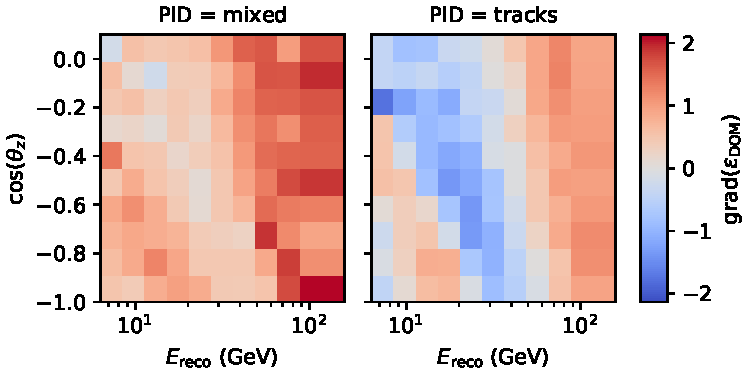
\includegraphics[width=0.9\linewidth]{figures/measurement/systematics/detector/hs_grad_dom_eff.pdf}
    \caption{Gradient of the relative bin count with respect to DOM efficiency.}
    \label{fig:dom-efficiency-slopes}
\end{figure}
A fundamental weakness of the linear fit treatment is that the fitted parameters are only valid for the choice of oscillation and flux parameters that they have been fitted with. In particular, there is a strong interaction between the DOM efficiency parameter and the $\Delta m^2_{31}$ oscillation parameter. As can be seen in \reffig{dom-efficiency-slopes}, the gradients of the relative bin counts with respect to DOM efficiency show a distinct imprint of the oscillation minimum. However, the location of this minimum depends on the current value of $\Delta m^2_{31}$, which causes a considerable bias if the value of $\Delta m^2_{31}$ at which the gradients are to be evaluated is different from the value at which they have been fitted. This is mitigated by running the fits at several values of $\Delta m^2_{31}$ covering the entire plausible range of this parameter, and interpolating all fit parameters with a piece-wise linear function between those points. As a result, all slopes and intercept values change as a function of the mass splitting. Although the interactions between detector systematic uncertainties and analysis parameters are not limited to the mass splitting, the bias produced as a result of the choice of other parameters was found to be much smaller and is therefore neglected in the three-flavor analysis. 

\subsection{Selection of Free Parameters}
\label{sec:std-osc-free-parameters}

The systematic uncertainties of the oscillation measurement consists of uncertainties on the properties of the detector, the neutrino flux, neutrino cross-sections, and atmospheric muon background. The effects of each of these uncertainties on the expectation values of the analysis histogram are parametrized by several parameters that are included as nuisance parameters during the fit with Gaussian priors when external constraints are available. The systematic uncertainties of the detector are described by five parameters for DOM efficiency, hole ice and bulk ice as described in \refsec{detector-unc}. Variations of the atmospheric neutrino flux are parametrized by varying the flux contributions of Pions and Kaons in each "Barr block" (see \refsec{flux_systs}) separately. Neutrino cross-section variations are modeled by varying the axial masses for resonant and quasi-elastic interactions, and by interpolating between the \textsc{GENIE} and \textsc{CSMS} cross-sections for DIS interactions as described in \refsec{xsec_systs}, with an additional 10\% error on the neutral-current contribution to reflect the uncertainty in the hadronization process. For the atmospheric muon background, both the total normalization and the spectral index of the flux can be varied.

When including all plausible sources of systematic uncertainties described above, the test statistic from \refeq{mod-chi2} would have to be optimized with respect to 28 nuisance parameters. Together with the two physics parameters, this would require an optimization in 30 dimensions to run the analysis. To reduce this computational burden, the potential bias and its significance that could plausibly be produced by each parameter is assessed, and the value of parameters that are found to have a negligible impact is fixed to its global best-fit value. The impact of each parameter is tested as follows: First, pseudo-data \emph{without} statistical fluctuations is produced from simulation where the value of the parameter to be tested is increased by $1\sigma$ if it has a Gaussian prior, or half-way to its upper boundary if it does not have a prior. The histograms are then fit back while keeping the parameter to be tested fixed at its nominal value. This fit is done once with the physics parameters ($\theta_{23}$ and $\Delta m^2_{31}$) fixed at the value that was used to create the pseudo-data, and once with the physics parameters left free. The difference in the test statistic $\chi^2_{\mathrm{mod}}$ between the free fit and the fit with physics parameters fixed to the truth, $\Delta \chi^2_{\mathrm{mod}}$, is referred to as \emph{mis-modeling}. The p-value of the mis-modeling, calculated under the assumption that it should follow a $\chi^2$-distribution with two degrees of freedom, can be interpreted as the significance with which the analysis would have rejected the true physics value \emph{solely} due to the exclusion of the parameter in question. This test neglects any global offset to the test statistic, since it would not affect the estimate of the confidence limits for the physics parameters.
\begin{figure}
    \centering
    %\missingfigure[figwidth=0.8\linewidth,figheight=0.7\linewidth]{Mis-modeling grid produced for one parameter in the mis-modeling ranking test.}
    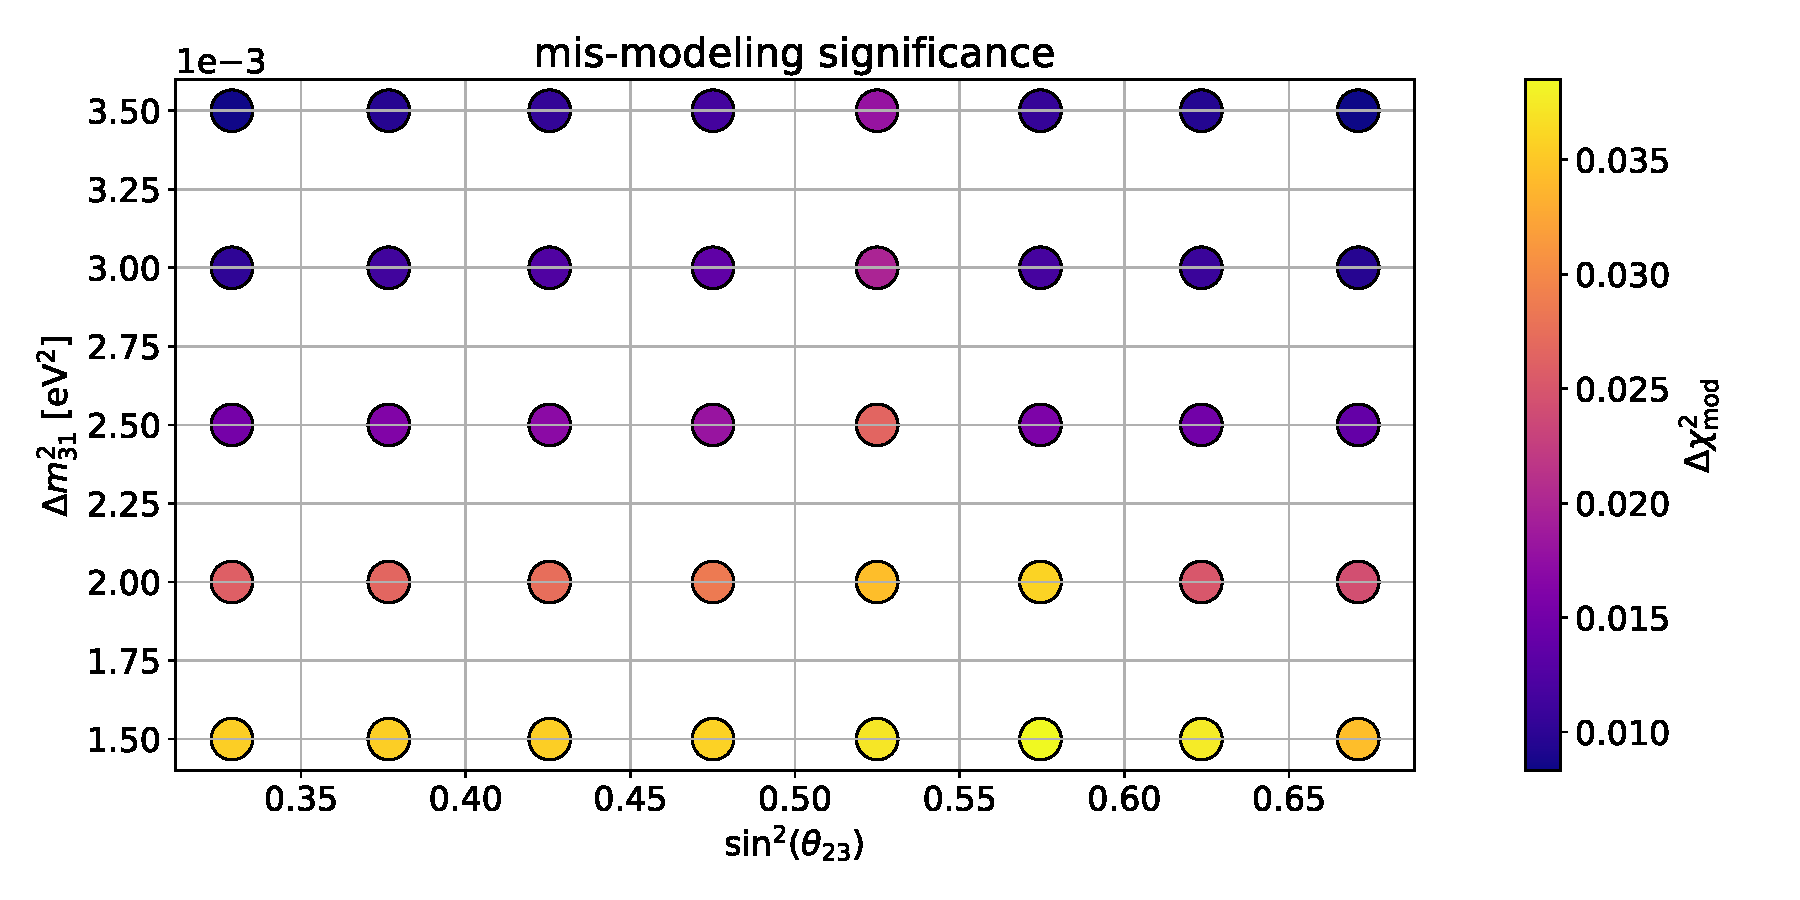
\includegraphics[width=\linewidth]{figures/measurement/three_flavor/asimov_test/systematic_impact_test-asimov_test-000015_GENIE_MA_QE.pdf}
    \caption{Grid of $\Delta \chi^2_{\mathrm{mod}}$ values showing the impact of the axial mass $M_A^{CCQE}$ being pulled by $1\sigma$.}
    \label{fig:systematic-impact-mismod-example}
\end{figure}
The test described above is repeated for a grid of true values of $\theta_{23}$ and $\Delta m^2_{31}$ that span the entire range of values that is not strongly excluded by other measurements, producing a value for $\Delta \chi^2_{\mathrm{mod}}$ at each point in the grid, as shown in \reffig{systematic-impact-mismod-example}. The largest value of $\Delta \chi^2_{\mathrm{mod}}$ of the entire grid produced for one parameter represents the \emph{maximum mis-modeling} for that parameter. Taking the maximum mismodeling for all parameters, one can produce a ranking of the impacts of all parameters of the analysis as shown in \reffig{systematic-impact-mismod-ranking}. Parameters for which the maximum mis-modeling lies below a conservatively chosen value of $\Delta \chi^2_{\mathrm{mod}} < 5\times10^{-3}$ are fixed to their global best-fit value in the analysis, reducing the total number of free parameters to 17. The complete list of all parameters of the analysis, their priors and their allowed ranges can be found in \reftab{sys-params-three-flavor} in the appendix.
\begin{figure}
    \centering
    %\missingfigure[figwidth=0.6\linewidth, figheight=0.8\linewidth]{Mis-modeling ranking for the three-flavor analysis.}
    \tikzsetnextfilename{three_flavor_mismod_ranking}%
\begin{tikzpicture}
    \begin{semilogxaxis}[
        tick label style = {font=\footnotesize\sffamily},
        xbar,
        xmin=2e-5,
        width=0.9\linewidth,
        height=1.1\linewidth,
        bar width=0.3cm,
        log origin=infty,
        %enlarge y limits=0.5,
        xlabel={maximum $\Delta \chi^2_\mathrm{mod}$},
        symbolic y coords={
            Barr $\bar{K}_\mathrm{Z}$, $\Delta \gamma_\mu$, Barr $\bar{K}_\mathrm{X}$, Barr $K_\mathrm{X}$, Barr $K_\mathrm{Z}$, $\pi^+/\pi^-$ ratio, Barr $\bar{K}_\mathrm{W}$, Barr $\bar{K}_\mathrm{Y}$, Barr $\pi_\mathrm{I}$, Barr $K_\mathrm{W}$, Barr $\pi_\mathrm{G}$, Barr $\pi_\mathrm{H}$, DIS CSMS, GENIE $M_A^{CCQE}$, Barr $\pi_\mathrm{A-F}$, NC norm, Barr $K_\mathrm{Y}$, ice scatter, ice abs, GENIE $M_A^{RES}$, $N_\mu$, $\Delta \gamma_{\nu}$, hole ice $p_1$, hole ice $p_0$, $N_\nu$, $\epsilon_\mathrm{DOM}$
        },
        ytick=data,
        xmajorgrids
    ]
        \addplot table [x=max_mismod, y=param_label, col sep=comma] {
            param_name, param_label, max_mismod
            barr_z_antiK, Barr $\bar{K}_\mathrm{Z}$, 0.0001
            delta_gamma_mu, $\Delta \gamma_\mu$, 0.0001
            barr_x_antiK, Barr $\bar{K}_\mathrm{X}$, 0.0001
            barr_x_K, Barr $K_\mathrm{X}$, 0.0001253586882728502
            barr_z_K, Barr $K_\mathrm{Z}$, 0.0005215688001167906
            pion_ratio, $\pi^+/\pi^-$ ratio, 0.0010014938724447354
            barr_w_antiK, Barr $\bar{K}_\mathrm{W}$, 0.0013617826249995284
            barr_y_antiK, Barr $\bar{K}_\mathrm{Y}$, 0.001784909483961046
            barr_i_Pi, Barr $\pi_\mathrm{I}$, 0.0028407893961021335
            barr_w_K, Barr $K_\mathrm{W}$, 0.009147508698163102
            barr_g_Pi, Barr $\pi_\mathrm{G}$, 0.013435565011888494
            barr_h_Pi, Barr $\pi_\mathrm{H}$, 0.014012540822907371
            dis_csms, DIS CSMS, 0.02336082345524751
            Genie_Ma_QE, GENIE $M_A^{CCQE}$, 0.038519249242069786
            barr_af_Pi, Barr $\pi_\mathrm{A-F}$, 0.04259356987935456
            nu_nc_norm, NC norm, 0.04460453331536404
            barr_y_K, Barr $K_\mathrm{Y}$, 0.06646024427532327
            ice_scatter, ice scatter, 0.0742952038753204
            ice_abs, ice abs, 0.10197443387707672
            Genie_Ma_RES, GENIE $M_A^{RES}$, 0.13818399497979877
            weight_scale, $N_\mu$, 0.4519687304055102
            delta_index, $\Delta \gamma_{\nu}$, 1.4839425295211388
            hole_ice_p1, hole ice $p_1$, 1.7423861973716477
            hole_ice_p0, hole ice $p_0$, 3.1929730025605423
            aeff_scale, $N_\nu$, 4.147319242014547
            dom_eff, $\epsilon_\mathrm{DOM}$, 16.08774037554603
        };
       % the [normalized] keyword is necessary because the axis uses symbolic y coordinates.
       % It is *critical* that there is no space before "[normalized]", and that "axis cs:" 
       % is used explicitly!
        \draw[thick, dashed] (axis cs:5e-3,{[normalized]\pgfkeysvalueof{/pgfplots/ymin}}) -- (axis cs:5e-3,{[normalized]\pgfkeysvalueof{/pgfplots/ymax}});
        \node[draw, thick, single arrow, shape border rotate=180, anchor=east, font=\footnotesize] at (axis cs:5e-3,{[normalized]0}) {fixed};
        \node[draw, thick, single arrow, anchor=west, font=\footnotesize] at (axis cs:5e-3,{[normalized]0}) {free};
    \end{semilogxaxis}
\end{tikzpicture}
    \caption{Ranking of $\Delta \chi^2_{\mathrm{mod}}$ values for all nuisance parameters considered for the three-flavor oscillation analysis.}
    \label{fig:systematic-impact-mismod-ranking}
\end{figure}

\section{Analysis Checks}
Before running the analysis on real data, its robustness is assessed on pseudo-data produced with simulated MC data sets. Once the robustness on pseudo-data has been established, the analysis is first run \emph{blindly}, that is, without showing the analyzer the results of the physics parameters and only revealing a set of goodness-of-fit variables that has been chosen in advance. Only when the values of these variables lie within the plausible range that can be expected from purely statistical fluctuations are the actual fit values of the measured parameters revealed. 

\subsection{Robustness of the minimization}
\label{sec:three-flavor-inject-recover-test}
The free fit of the physics parameters $\theta_{23}$ and $\Delta m^2_{31}$ is run separately once for the lower octant ($\theta_{23} < 45^\circ$) and once for the upper octant ($\theta_{23} > 45^\circ$) to break the degeneracy between the octants. Each fit uses the \textsc{scipy}\cite{2020SciPy-NMeth} implementation of the \textsc{L-BFGS-B} algorithm\cite{l-bfgs-b} to find the parameter values that minimize the $\chi^2_{\mathrm{mod}}$ test statistic. To ensure that the minimization will always converge to the global optimum for any true value of the physics parameters, pseudo-data without statistical fluctuations (also referred to as an \emph{Asimov} test set) is produced on a grid spanning all values that are not strongly excluded by other experiments and a fit is run for each grid point. Since there are no statistical fluctuations, the fit is expected to always converge exactly to the injected true value. As can be seen in the result shown in \reffig{three-flavor-asimov}, the convergence of the minimizer is robust everywhere. 
\begin{figure}
    \centering
    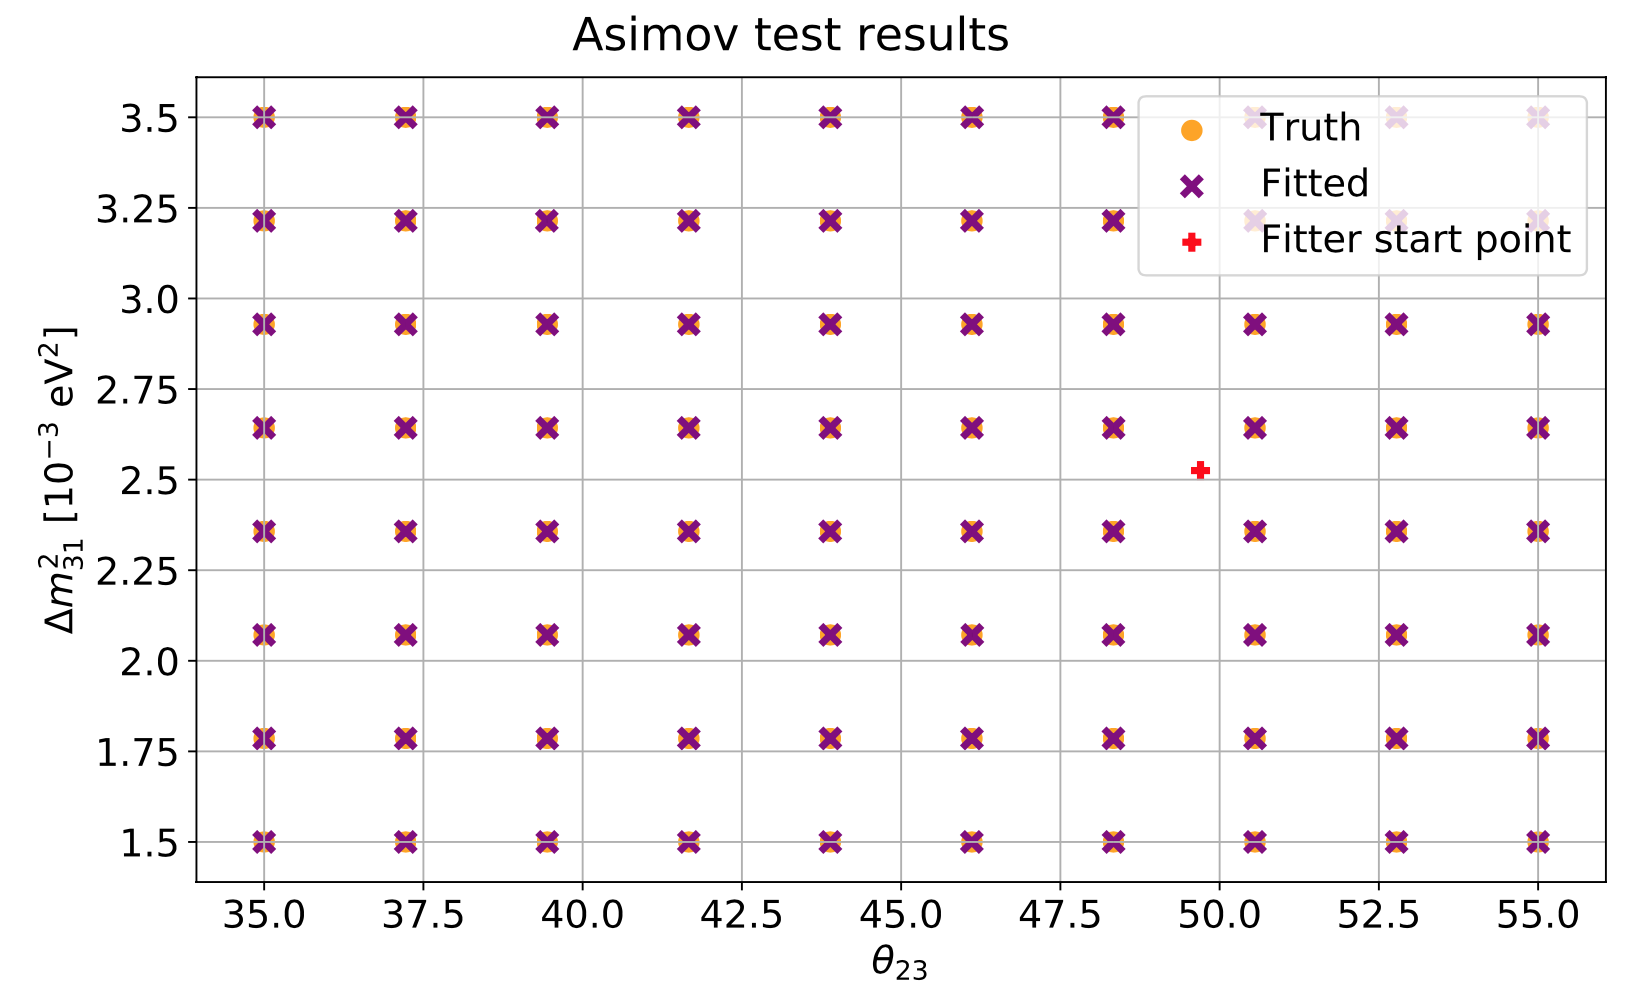
\includegraphics[width=0.9\linewidth]{figures/measurement/three_flavor/asimov_test/inject_recover_map.png}
    \caption{Asimov inject/recover test result for the three-flavor oscillation analysis.}
    \label{fig:three-flavor-asimov}
\end{figure}

\subsection{Ensemble tests}
\label{sec:three-flavor-ensemble}
To get expected distributions of the test statistic and parameter fluctuations, the analysis is run on an ensemble of fluctuated pseudodata. For every trial of the ensemble, the expectation value in every analysis bin is first drawn from a normal distribution centered on the MC expectation with a standard deviation corresponding to the MC uncertainty. Using these sampled expectation values, the bin count is drawn from a Poisson distribution independently in every bin. This sampling scheme ensures that the fluctuations reflect both the MC uncertainty and the Poisson fluctuations expected in data. A free fit is run on every trial, producing a set of best-fit parameters, a value for the total $\Delta \chi^2_{\mathrm{mod}}$ test statistic, as well as the contribution of each bin in the analysis histogram to this total value.
%The distribution for the fit parameters and their pull from their injected values from the ensemble is shown in \reffig{three-flavor-ensemble-param}. The distributions for all parameters are centered on the injected value, demonstrating that the fit is behaving robustly under the expected fluctuations. 

% \begin{figure} 
%     \centering
%     \begin{subfigure}[t]{0.99\textwidth}
%         \centering
%         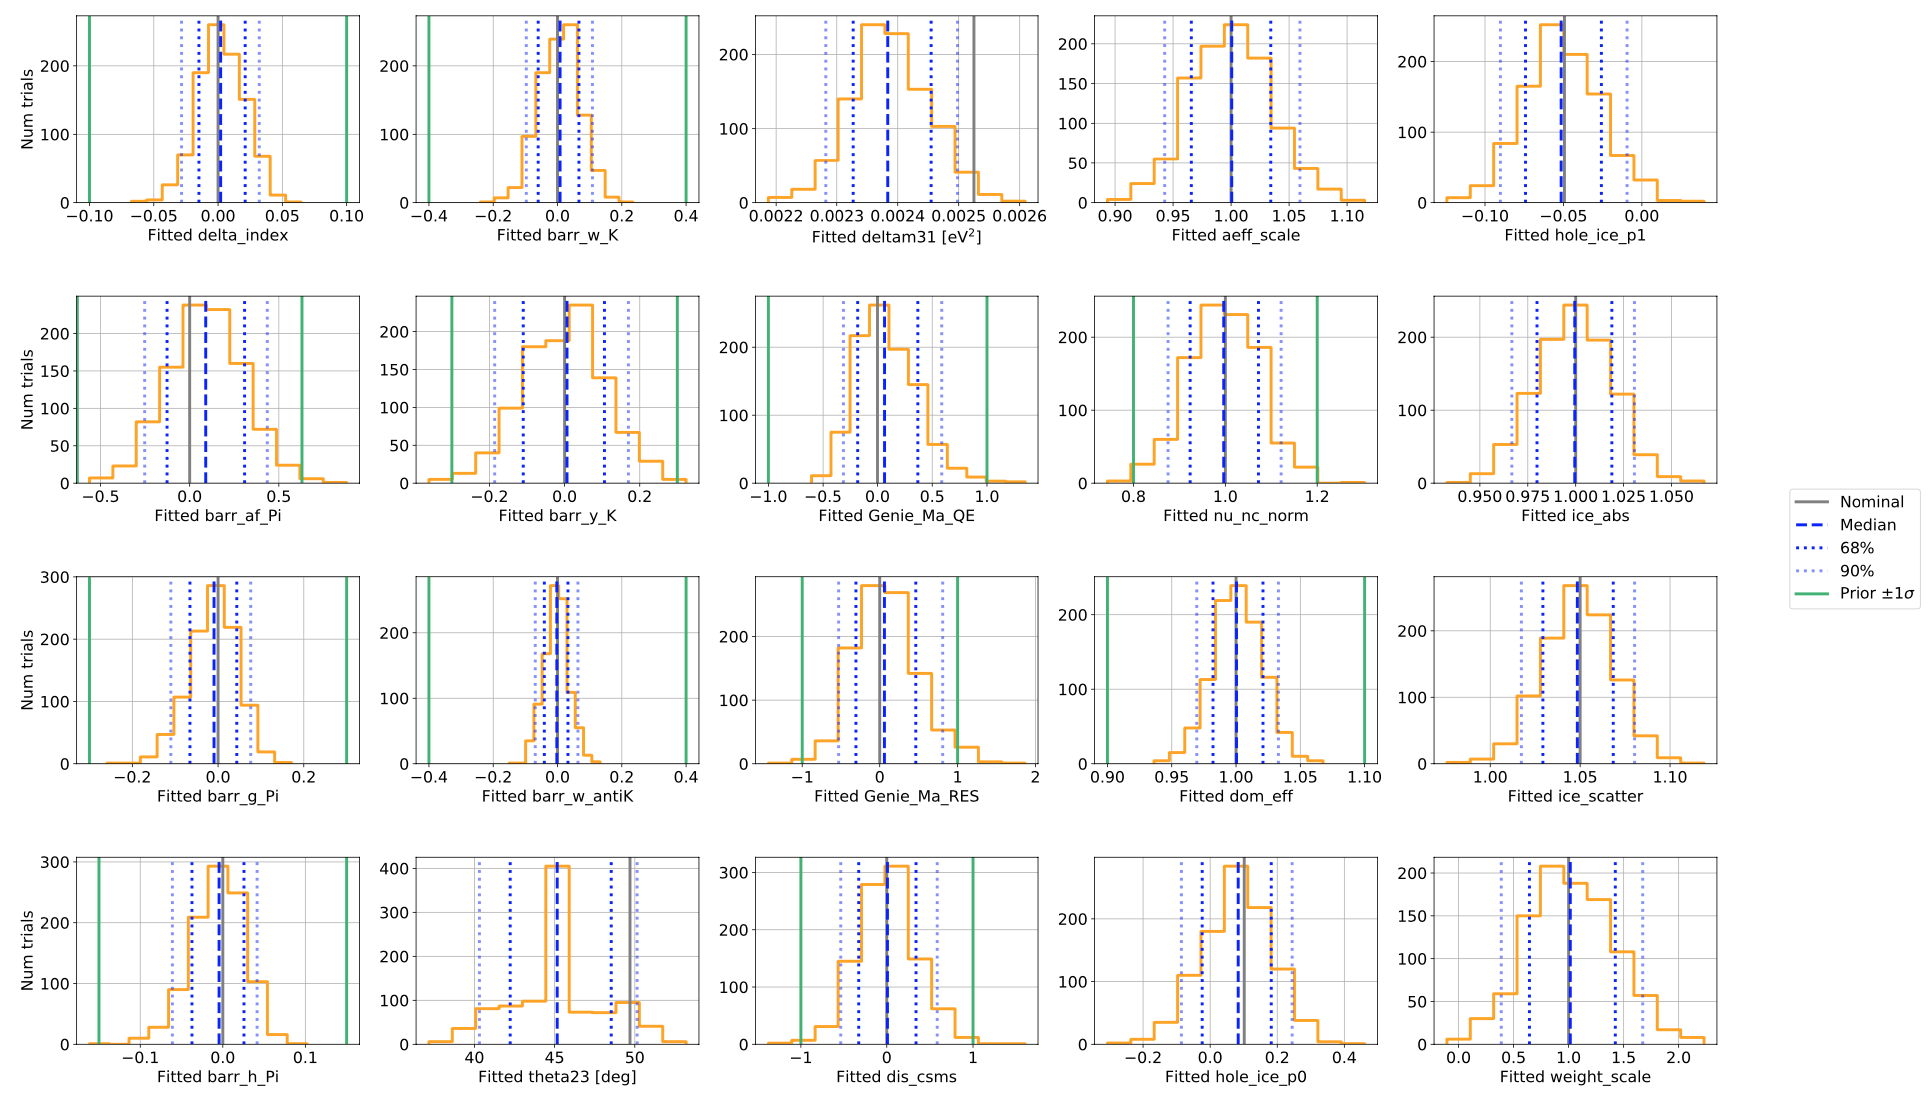
\includegraphics[width=0.99\textwidth]{figures/measurement/three_flavor/ensemble_pre_fit/ensemble_fitdist.png}
%     \end{subfigure}
%     \begin{subfigure}[t]{0.65\textwidth}
%         \centering
%         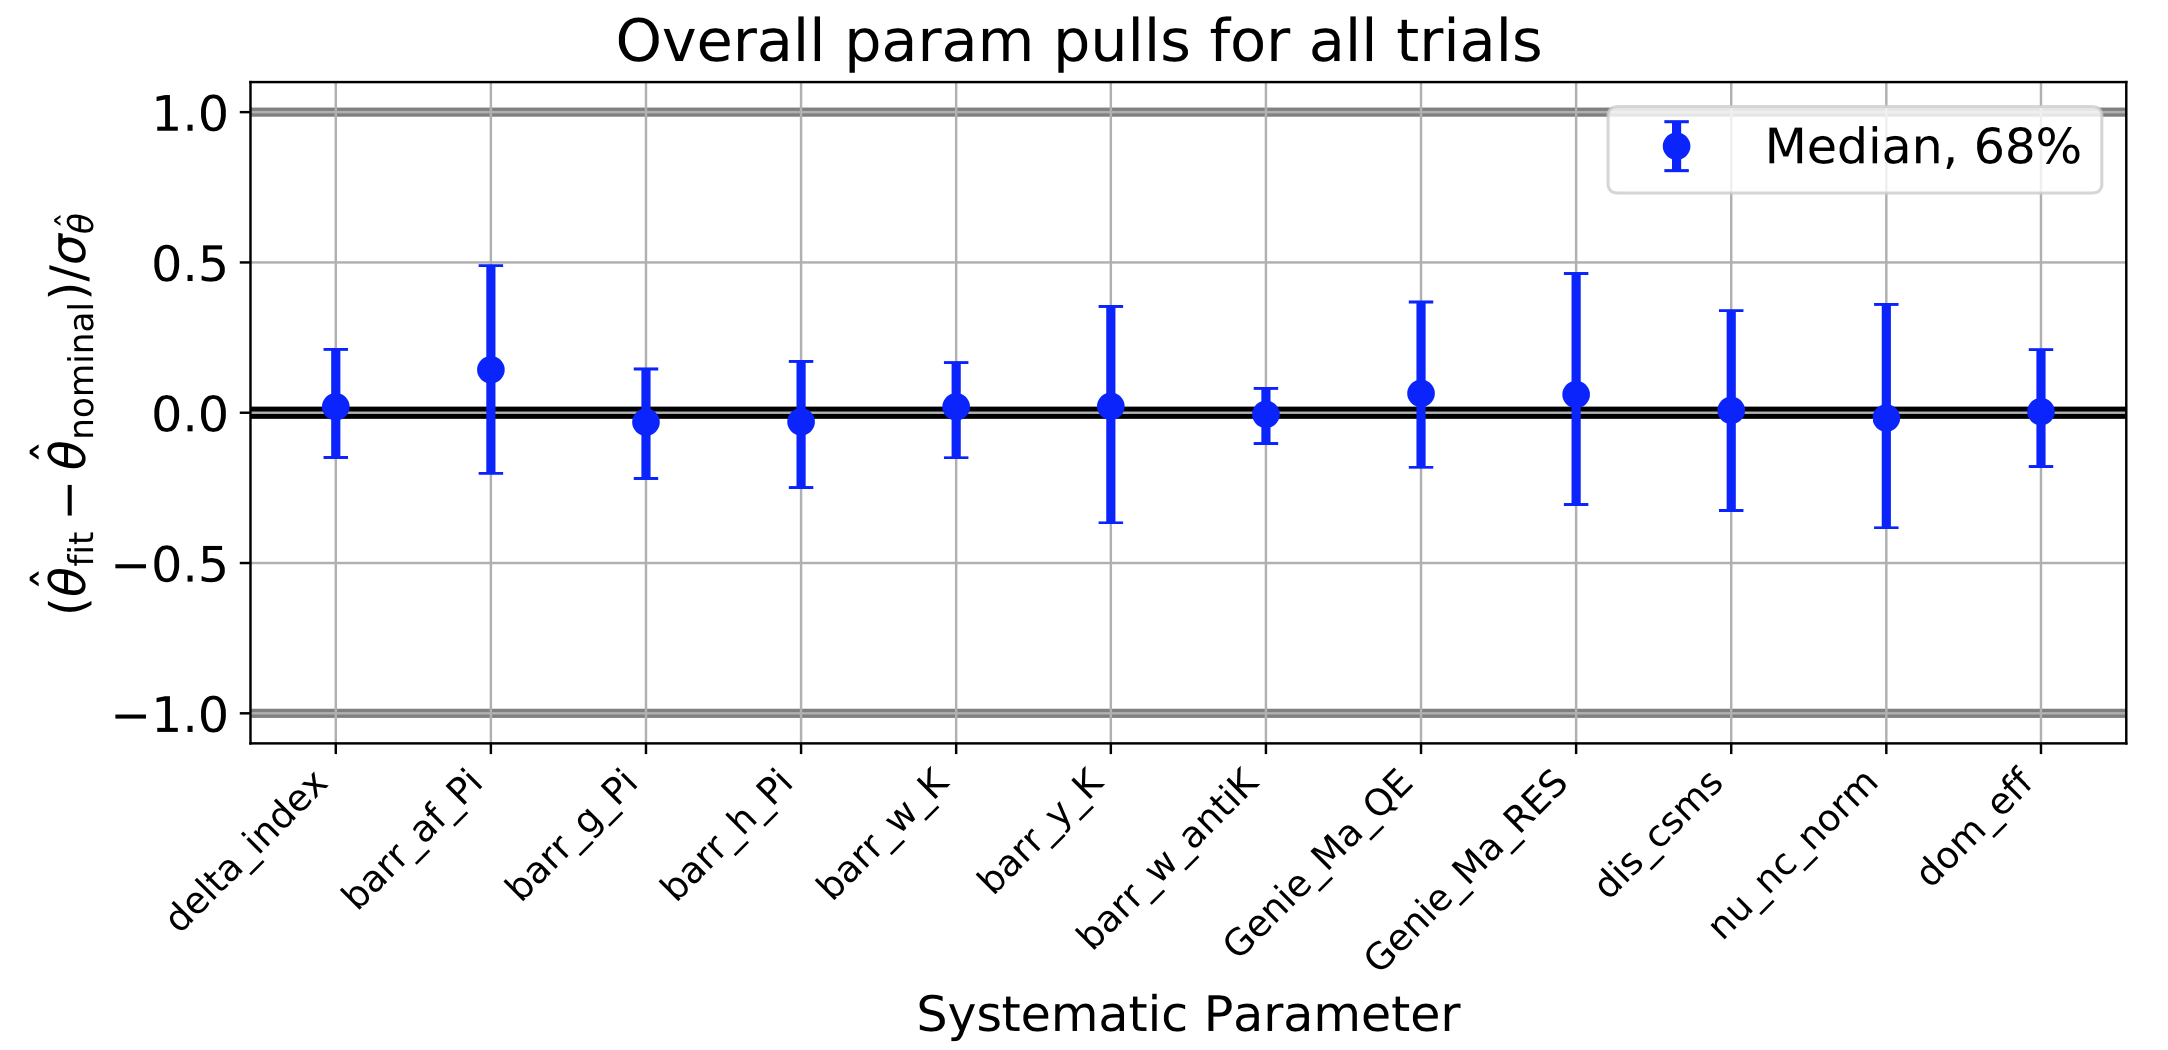
\includegraphics[width=0.99\textwidth]{figures/measurement/three_flavor/ensemble_pre_fit/ensemble_pull.png}  
%     \end{subfigure}
%   \caption{Distributions of fitted values of each parameter considered in the three-flavor analysis (top), and their corresponding pulls from nominal (bottom).
%   \label{fig:three-flavor-ensemble-param}}
% \end{figure}


\subsubsection{Goodness of Fit}

Before looking at the best fit parameters of the real data fit, the goodness of fit is assessed using the total and bin-wise test statistic distributions. The distribution of the test statistic acquired from the ensemble described in \refsec{three-flavor-ensemble} is shown in \reffig{three-flavor-ts-ensemble} together with the observed test statistic from real data. The observed test statistic is found to lie very well within the expectation with a p-value of 32\%. The bin-wise contribution and the test statistic and its expected distribution are shown in \reffig{three-flavor-binwise-ts}. The histogram shows no apparent regions of particularly bad agreement between the data and the MC expectation, and the distribution of the bin-wise test statistic is in agreement with the distribution expected from pseudo-data trials.

\begin{figure}
    \centering
    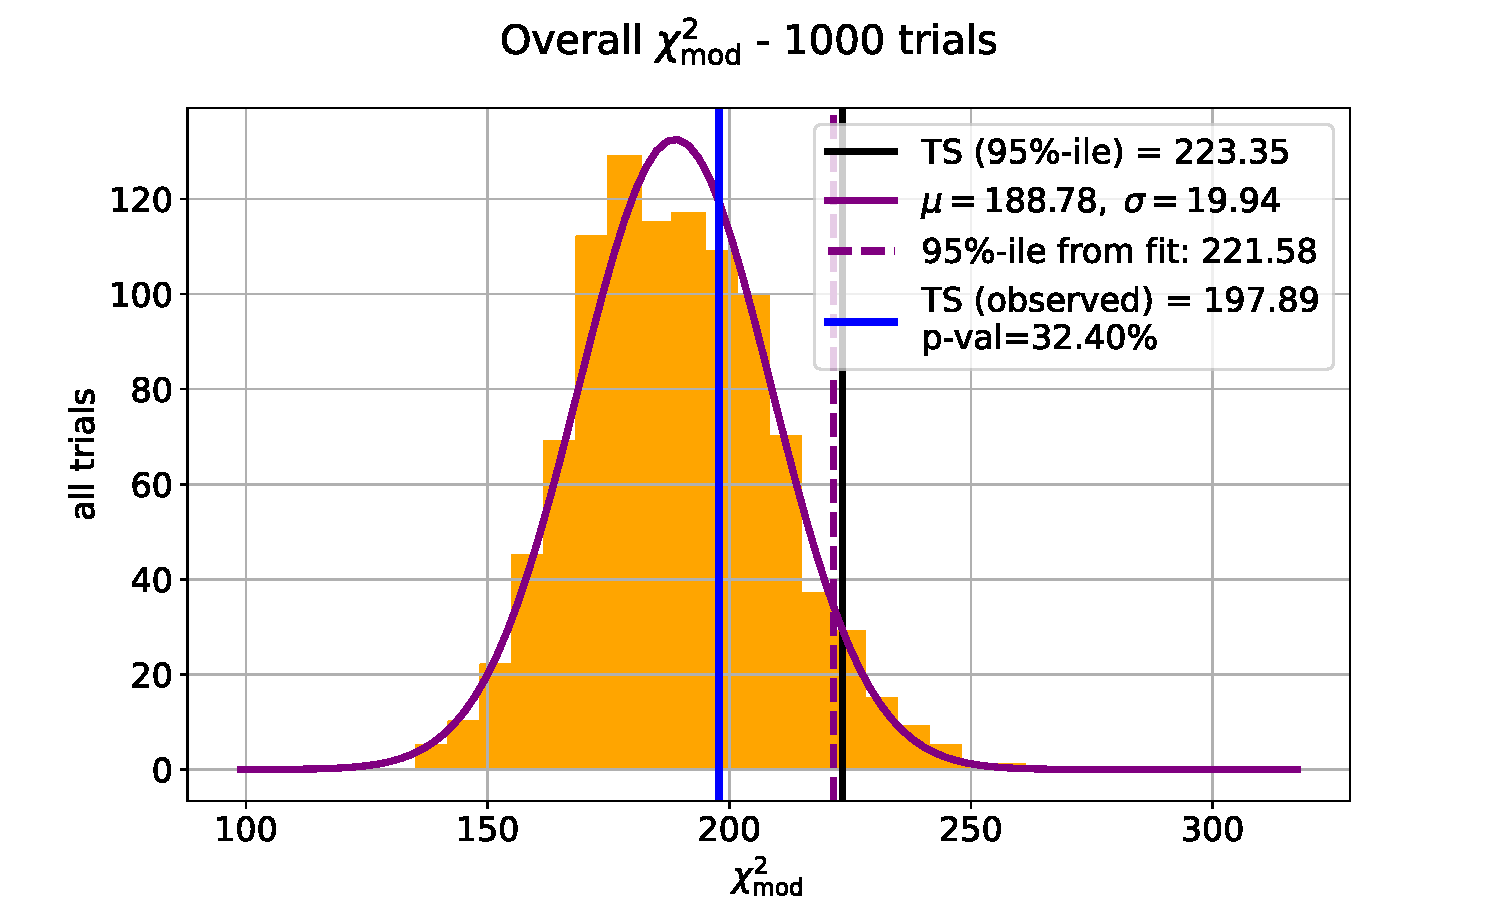
\includegraphics[width=0.8\linewidth]{figures/measurement/three_flavor/ensemble_pre_fit/overall_ts_wings_trials.pdf}
    \caption{Observed test statistic value of the three-flavor oscillation analysis compared to expected distribution from ensemble.}
    \label{fig:three-flavor-ts-ensemble}
\end{figure}

\begin{figure*}
    \centering
    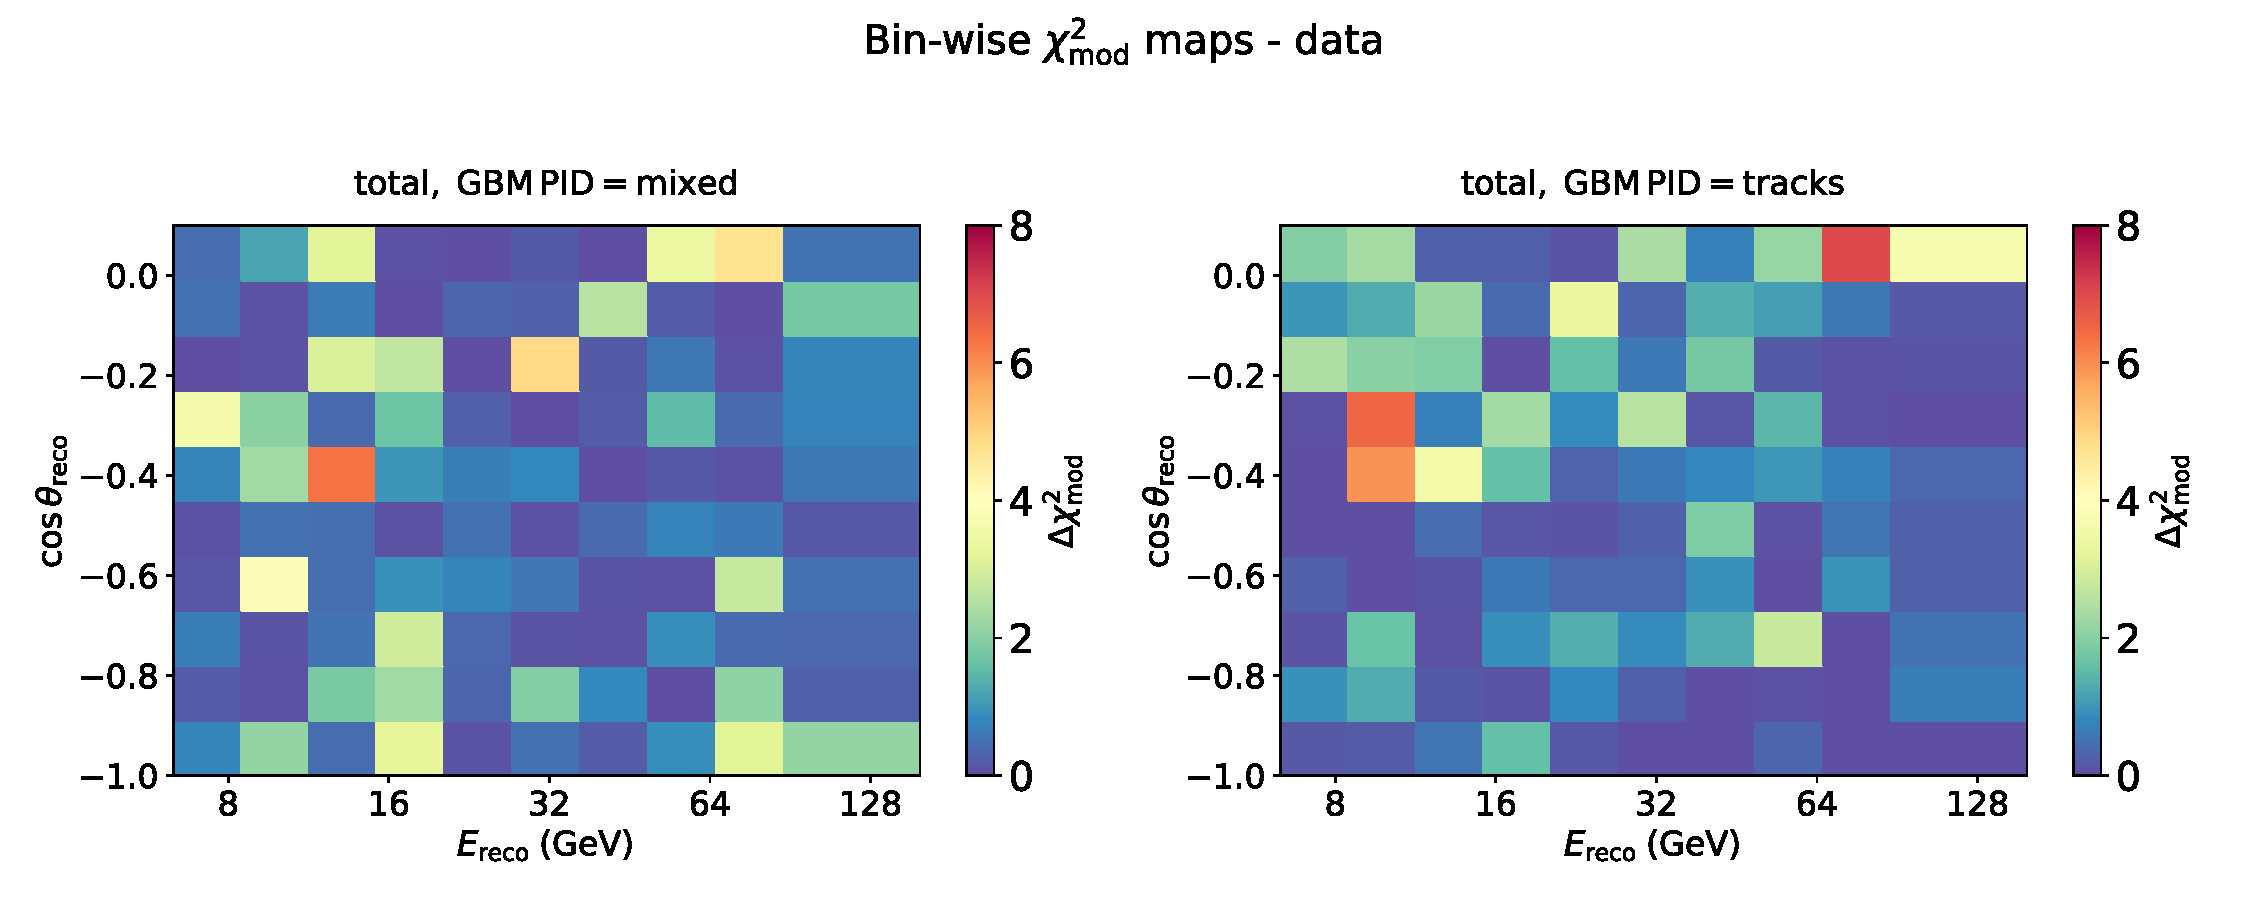
\includegraphics[height=0.22\linewidth,trim={0 0 0 1.5cm},clip]{figures/measurement/three_flavor/ensemble_pre_fit/real_fit_binwise_pulls_pre_bugfix.pdf}
    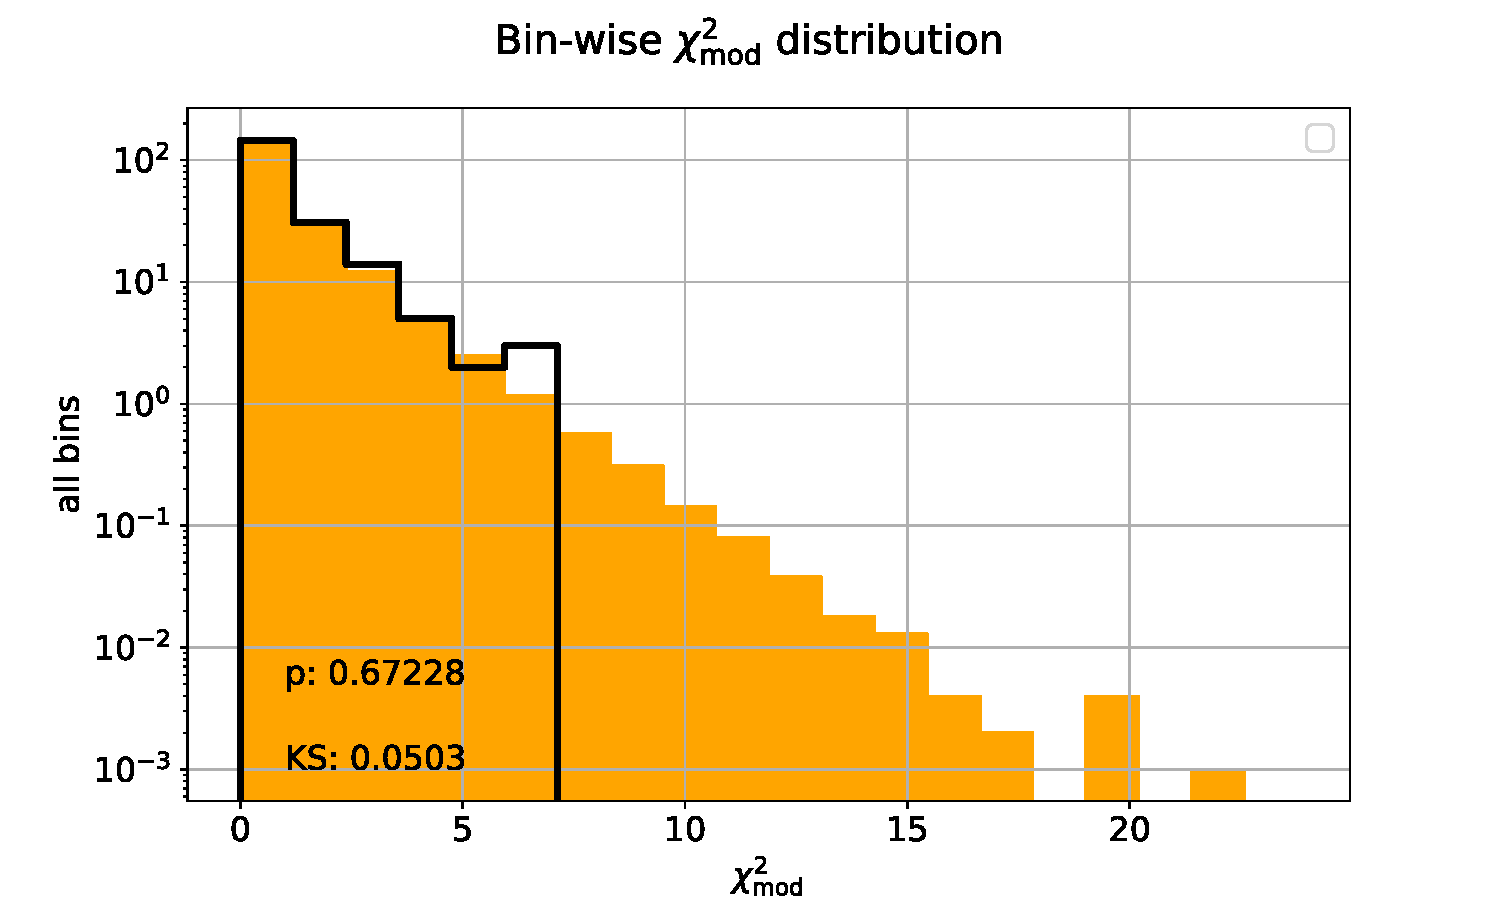
\includegraphics[height=0.22\linewidth]{figures/measurement/three_flavor/ensemble_pre_fit/binwise_ts_wings_trials.pdf}
    \caption{Contribution of every bin to the over-all test statistic in the three-flavor analysis (left) and their observed distribution compared to the expected distribution from pseudo-data trials (right).}
    \label{fig:three-flavor-binwise-ts}
\end{figure*}

\subsubsection{Test for un-physical mixing}
If the real data contains an under-fluctuation in the oscillation valley, it is possible that the fit prefers more than maximal $\nu_\mu$ disappearance, which is physically not possible. This tendency to fit unphysical magnitudes of $\nu_\mu$ disappearance is tested by running a fit in which the oscillation probabilities are calculated with a simplified two-flavor equation in which the scale of the oscillation, $\sin^2(2\theta_{23})$\todo{explain this simplification in the theory section and link here}, is replaced with a scaling factor that is allowed to float freely even to unphysical values where $\sin^2(2\theta_{23}) > 1$. If the true mixing angle is $\theta_{23}=45^\circ$, it is expected that such unphysical best-fit values can occur solely due to random Poisson fluctuations of the data. To quantify this expectation, another ensemble of trials is produced where the injected true mixing is maximal. The two flavor analysis is run on each trial to produce a distribution of expected values that is shown in \reffig{two-flavor-ensemble}. The results show that, while the real data fit does indeed prefer a slightly unphysical $\nu_\mu$ disappearance, this preference still lies well within the expectation if the true mixing was assumed to be maximal.

\begin{figure}
    \centering
    \tikzsetnextfilename{two_flavor_ensemble_threshold_anotated}%
\begin{tikzpicture}
    \node[above right, inner sep=0] (image) at (0,0) {
        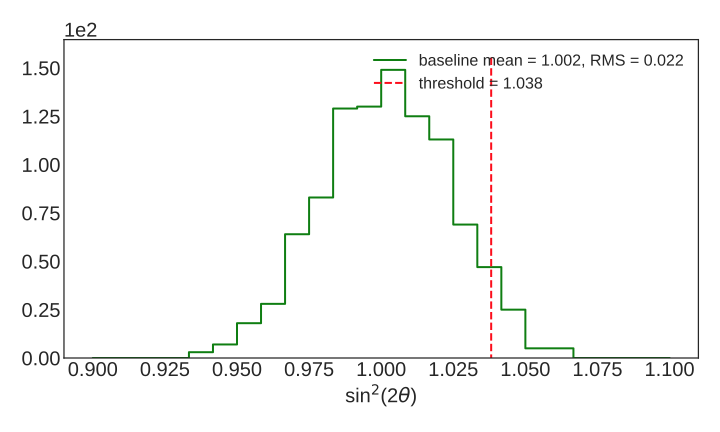
\includegraphics[width=0.8\linewidth]{figures/measurement/three_flavor/ensemble_pre_fit/two_flav_ensemble_threshold.png}
    };
    % Create scope where axes are the plot coordinates
    \begin{scope}[
        x={($0.4*(image.south east)$)},
        y={($0.45*(image.north west)$)},
        shift={($0.13*(image.south east) + 0.17*(image.north west)$)}
    ]
        % Grid
        %\draw[darkgray,step=.25] (0,0) grid (2,1.5);
        % x-coordinates start at 0.9 and one unit = 0.1
        \draw (1.23, 0) -- node [sloped, font=\footnotesize, anchor=south] {observed $=1.023$} (1.23, 1.3);
    \end{scope}
\end{tikzpicture}
    %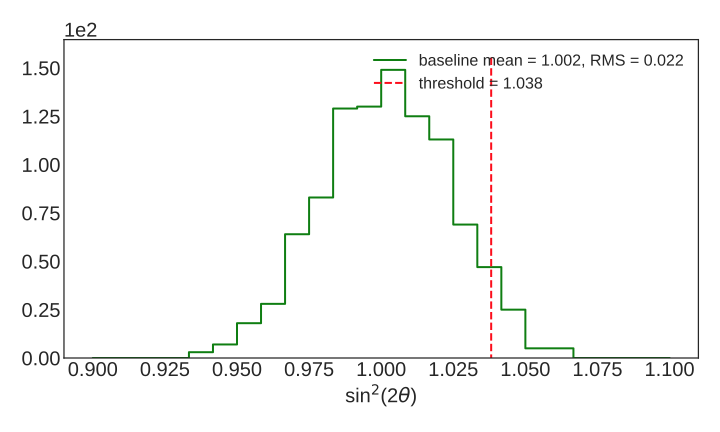
\includegraphics[width=0.8\linewidth]{figures/measurement/three_flavor/ensemble_pre_fit/two_flav_ensemble_threshold.png}
    \caption{Observed best fit values of the two-flavor fit compared to the distribution from pseudo-data trials.}
    \label{fig:two-flavor-ensemble}
\end{figure}

\subsubsection{Likelihood Coverage}

When drawing the 90\% exclusion contour shown in \reffig{real_data_contour_three_flavor}, it is assumed that Wilks' theorem holds, that is, the distribution of the test statistic follows a $\chi^2$ distribution with two degrees of freedom. If more than 90\% of repeated measurements fall below the 90\% threshold, the likelihood is said to be \emph{over-covering}. In the reverse case where fewer than 90\% of repeated measurements fall below the 90\% threshold, the likelihood is said to be \emph{under-covering}. The coverage of the likelihood may change depending on the assumed true parameter values. For this measurement in particular, it is expected that the likelihood should over-cover near maximal mixing, because the mixing angle can no longer provide a full degree of freedom. To test the coverage for particular values of $\theta_{23}$ and $\Delta m^2_{31}$, pseudo-data is generated where these values are injected as true values. The bin counts of the pseudo-data are Poisson-fluctuated to create an ensemble of trials. Then, one free fit is run and another fit where the physics parameters are fixed to their true values. The coverage is then evaluated by counting the fraction of trials for which $\Delta \chi^2_{\mathrm{mod}}$ between these two fits is smaller than the 90\% threshold given by Wilks' theorem. The results are shown in \reffig{three-flavor-coverage} for a range of points in mixing angle and mass splitting. As expected, the likelihood is over-covering near maximal mixing, while there is very little dependence of the coverage on the mass splitting. The likelihood is over-covering for all points in mass splitting in the right panel of \reffig{three-flavor-coverage}, because the injected mixing angle was at the best fit point of the analysis, which is very close to maximal. In conclusion, the 90\% contours shown in \reffig{real_data_contour_three_flavor} are slightly over-conservative in the region close to maximal mixing.

\begin{figure*}
    \centering
    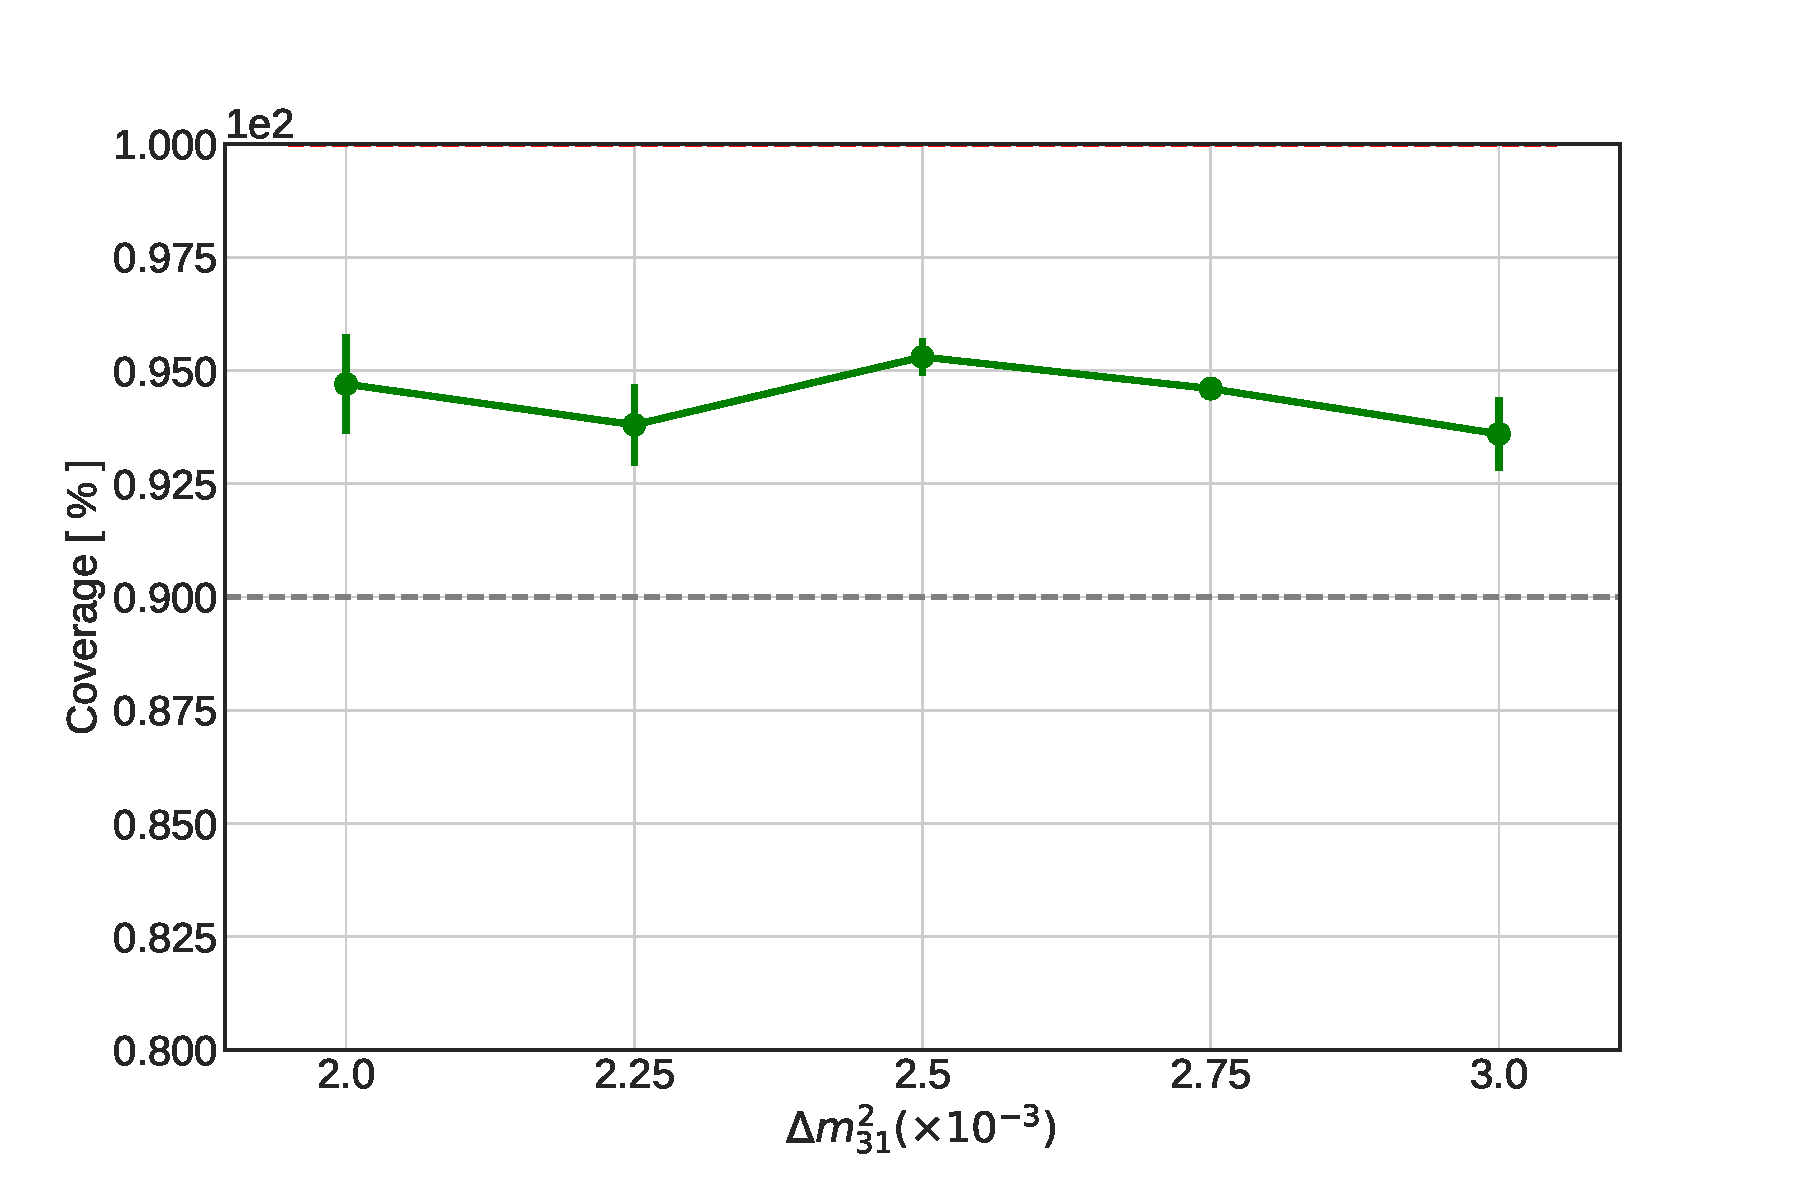
\includegraphics[width=0.45\linewidth]{figures/measurement/three_flavor/coverage_test/coverage_dm_v3.pdf}
    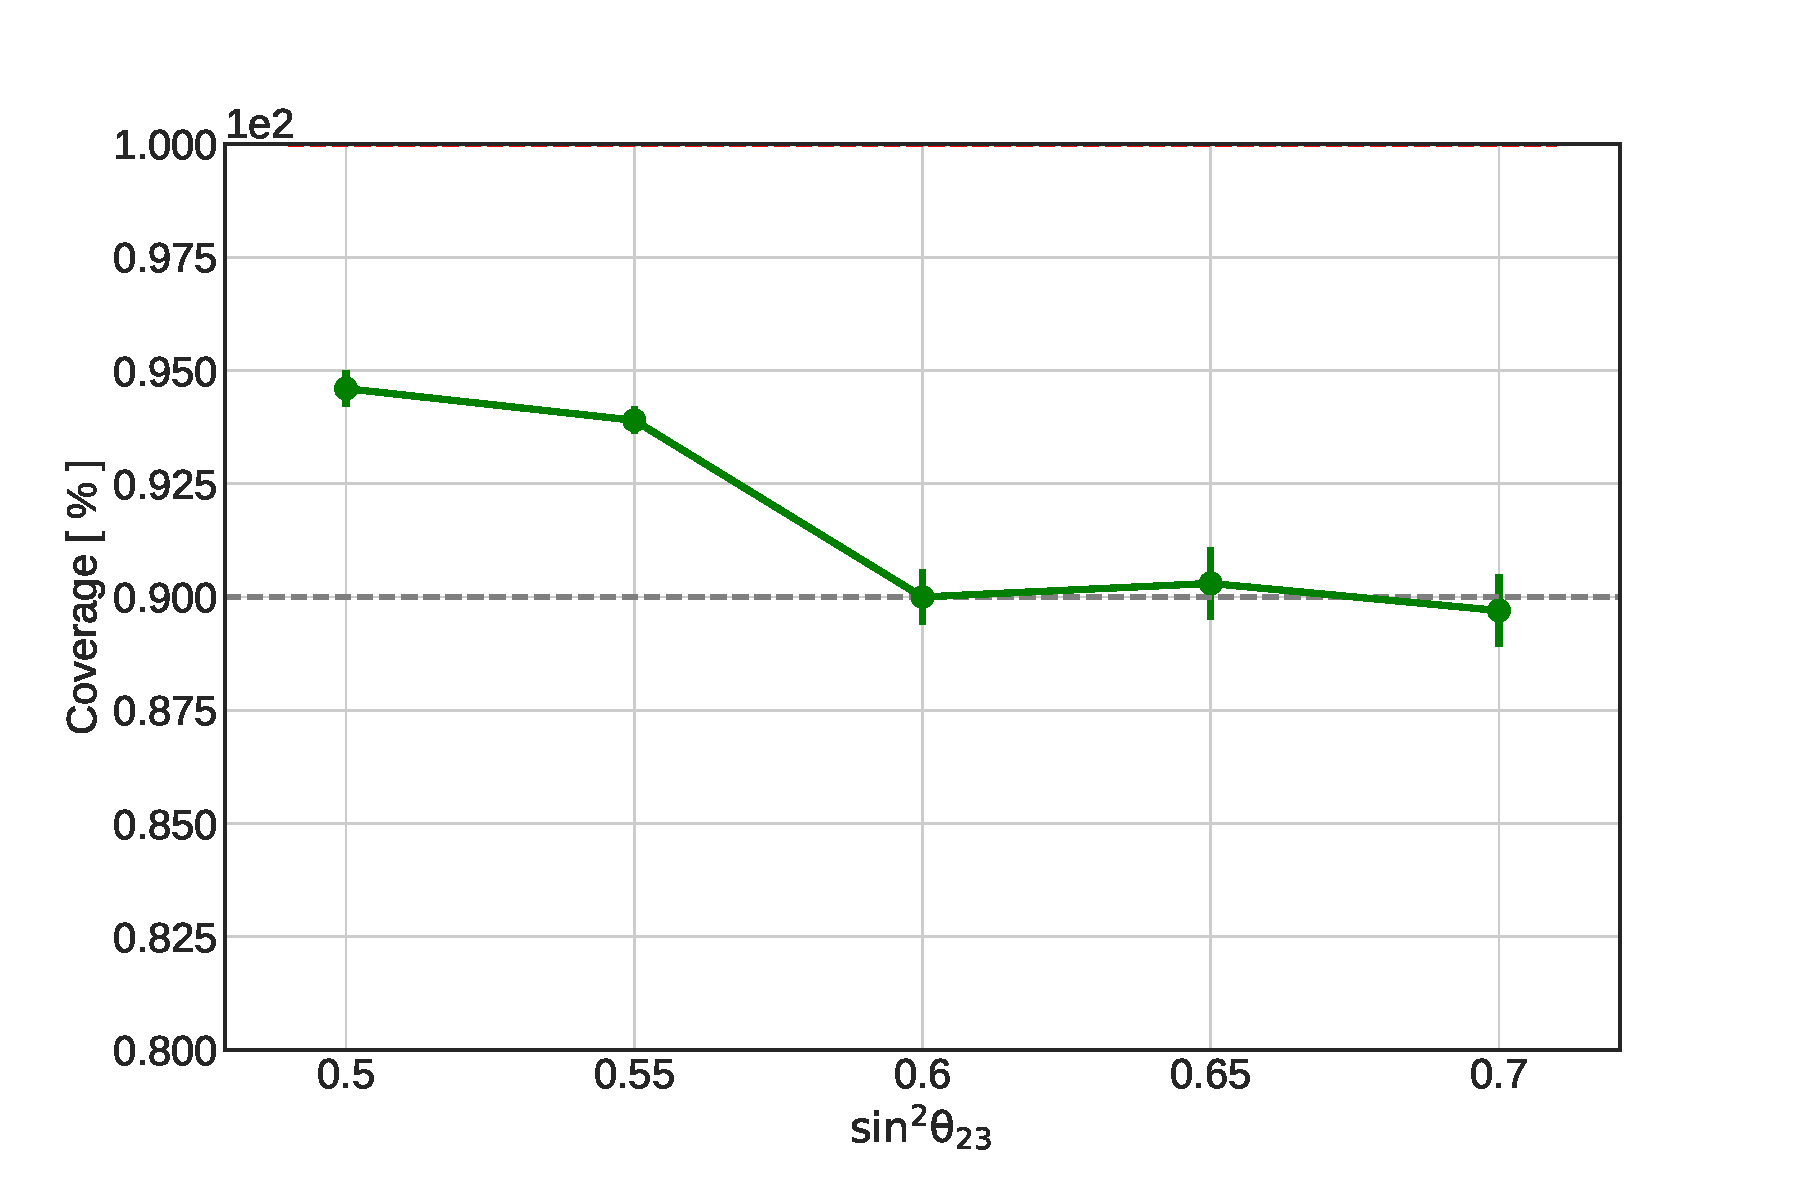
\includegraphics[width=0.45\linewidth]{figures/measurement/three_flavor/coverage_test/coverage_t23_v3.pdf}
    \caption{Fraction of trials below the 90\% threshold expected from Wilks' theorem for a range of points in mass splitting (left) and mixing angle (right).}
    \label{fig:three-flavor-coverage}
\end{figure*}

\subsubsection{Seasonal Stability}

Ensembles of trials also provide a way to ensure that the variations of the values of nuisance parameters between seasons lie within the expectation of pure statistical fluctuations. A program is written for this purpose that produces an ensemble of pseudo-data, in which every trial simulates one year of detector exposure. The program then histograms the best-fit values of each parameter while subtracting the best-fit point to give an expectation for the size of the fluctuation in that parameter between statistically independent years, and overlays the fit results from the different seasons of real data. This procedure protects the blindness of the analyzers because it never reveals the true best-fit points that have been subtracted from each histogram. The results show no sign of fluctuation between seasons that could not be readily explained by pure Poisson fluctuations.


\section{Results}

To prevent biasing the result due to psychological effects such as the well-known confirmation bias, the results of the analysis are revealed by scripts of code that only print out goodness-of-fit variables such as the test statistic and the parameter pulls to the console while hiding the physics result from the analyzers. Only after all establishing a good fit without extraordinary parameter pulls, the code reveals the final physics result and likelihood contours that are discussed in this section.

\subsection{Measured Nuisance Parameter Values}
The results for all nuisance parameters are shown in \reftab{nuisance_params_fittedval}. The pull values show that all parameters fit comfortably within $1\sigma$ of their defined priors. The fit prefers a slightly harder cosmic ray spectrum and a larger muon background than initially expected. The optical efficiency of the DOMs fits to a slightly larger value than nominal with 106\%, while the ice properties stay very close to their initial values.

%The hole ice parameters prefer less acceptance of photons entering the DOMs directly from below, and the shape of their corresponding acceptance curve is close to the best fit result from LED flasher studies\todo{cite hole ice flasher studies} as shown in \reffig{hole-ice-flasher-comparison-three-flavor}.

\begin{table}
    \centering
    \caption{Fitted values of all nuisance parameters from the all-season three-flavor fit. The pull of the best fit value is shown for parameters with a defined prior.}
    \label{tab:nuisance_params_fittedval}
    \begin{tabular}{clSS} \toprule
        category & Parameter  & {Best Fit Value} &  {Pull ($\sigma$)} \\ \midrule
        \multirow{7}{5em}{$\nu$ flux}& $\Delta \gamma_\nu$ & 0.065 & 0.65 \\
        & Barr $\pi_\mathrm{AF}$ & 0.233  & 0.369 \\
        & Barr $\pi_\mathrm{G}$ & -0.055  & -0.183 \\
        & Barr $\pi_\mathrm{H}$ & -0.0179  & -0.119 \\
        & Barr $K_\mathrm{W}$ & 0.0824  & 0.206 \\
        & Barr $K_\mathrm{Y}$ & 0.106  & 0.355 \\
        & Barr $\bar{K}_\mathrm{W}$ & -0.009  & -0.0224 \\ \midrule
        \multirow{4}{5em}{cross-section}& $M_{A}^{CCQE}$ &  0.0283 & 0.0283 \\
        & $M_{A}^{CCRES}$ & 0.572 & 0.572 \\
        & DIS CSMS & 0.0379  & 0.0379 \\ 
        & NC norm & 1.13 &  0.633 \\ \midrule
        \multirow{5}{5em}{detector systematics} & $\epsilon_\mathrm{DOM}$ & 1.06  & 0.625 \\
        & hole ice $p_0$ & -0.269  &  \\
        & hole ice $p_1$ & -0.041  &  \\
        & ice absorption & 0.974  &  \\
        & ice scattering & 0.989 &  \\ \midrule
        \multirow{2}{5em}{norm}& $N_\mu$ & 1.39  &  \\
        & $N_\nu$ & 0.824 &  \\
        \bottomrule
    \end{tabular}
\end{table}

The best-fit point of the hole ice parameters $p_0$ and $p_1$ is close to the results of the LED flasher fits shown in \reffig{hole-ice-parametrization}. The resulting light acceptance curve is shown in \reffig{hole-ice-bfp-comparison} compared to the curves produced by \emph{in-situ} LED calibration studies. The result of the three-flavor oscillation fit agrees with the LED calibration result in preferring a lower forward acceptance than the baseline hole ice model.
\begin{figure}
    \centering
    \tikzsetnextfilename{hole_ice_best_fit_point_comparison}%
\begin{tikzpicture}

\pgfplotstableread{figures/measurement/systematics/detector/hole_ice/all_acceptance_curves.csv}\acceptancecurves

\begin{axis}[
        width=0.8\linewidth, height=0.5\linewidth,
		xmajorgrids, ymajorgrids,
		xlabel=$\cos(\eta)$, ylabel=relative optical efficiency,
		legend style={at={(0.02,0.95)}, anchor=north west},
        ytick distance=0.2,
	]
    \addplot[black, very thick] table [x=cos_theta, y=bfp_three_flav] \acceptancecurves;
    \addlegendentry{best fit point}

    \addplot[black, thick, dashed] table [x=cos_theta, y=baseline] \acceptancecurves;
    \addlegendentry{baseline}
    
    \addplot[bluishgreen, thick] table [x=cos_theta, y=all] \acceptancecurves;
    \addlegendentry{combined LEDs}
    
    \addplot[bluishgreen, thick, dashed] table [x=cos_theta, y=tilted] \acceptancecurves;
    \addlegendentry{tilted LEDs}

    \addplot[bluishgreen, thick, dotted] table [x=cos_theta, y=horizontal] \acceptancecurves;
    \addlegendentry{horizontal LEDs}
	
\end{axis}
\end{tikzpicture}
    \caption{Angular acceptance curves corresponding to the best fit point of the three flavor and sterile oscillation fits compared to the results of LED flasher calibration studies.}
    \label{fig:hole-ice-bfp-comparison}
\end{figure}


\subsection{Oscillation parameters}
The fitted values for the three-flavor oscillation parameters are
\begin{align*}
    \sin^2\theta_{23} &= 0.507_{-0.053}^{+0.050}\\
    \Delta m^2_{32} &= 2.42_{-0.75}^{+0.77} \times10^{-3}\;\mathrm{eV}^2.
\end{align*}
The 90\% C.L. allowed region for these parameters is shown in \reffig{real_data_contour_three_flavor} compared to measurements from other experiments. The observed confidence limits for $\theta_{23}$ are slightly smaller than what would be expected from a likelihood scan over Asimov pseudo-data that was produced at the best fit point. To make sure that this is compatible with random fluctuations, the likelihood is profiled over $\sin^2(\theta_{23})$ for 100 pseudo-data trials including both Gaussian fluctuations that emulate the MC uncertainty and Poisson fluctuation for the data uncertainty. \reffig{mixing_brazil_band_three_flavor} shows the 68\% (90\%) intervals of the test statistic at each point of the scan over all trials. The observed contour is fully contained in the 68\% band, demonstrating that the narrowed 90\% range for $\theta_{23}$ is fully compatible with expected data fluctuations. The contribution of each category of systematic uncertainties shown in \reftab{nuisance_params_fittedval} to the total uncertainty is shown in \reftab{error_budget}. The values show that the largest contribution to the total systematic uncertainty of the analysis is by far the uncertainty on the detector properties. Overall, the result provides constraints on the atmospheric mass splitting and mixing angle that are the most stringent in its class of experiments and are competitive with those from accelerator experiments.
\begin{margintable}
    \caption{Contribution of each category of systematic uncertainties to the total error budget in each physics parameter.}
    \label{tab:error_budget}
    \begin{tabular}{p{4em}SS}
        \toprule
        & \multicolumn{2}{c}{error contrib. (\%)} \\ \cmidrule{2-3}
        category & $\Delta m^{2}_{32}$ & $\sin^{2}\theta_{23}$  \\
        \midrule
        $\mu$ norm       & 1.8   & 1.1    \\
        $\nu$ norm       & 1.0   & 0.4    \\
        detector         & 33.6  & 10.6   \\
        $\nu$ flux       & 5.4   & 1.4    \\
        cross-section    & 6.8   & 0.3    \\
        \bottomrule
    \end{tabular}
\end{margintable}

\begin{figure}
    \centering
    %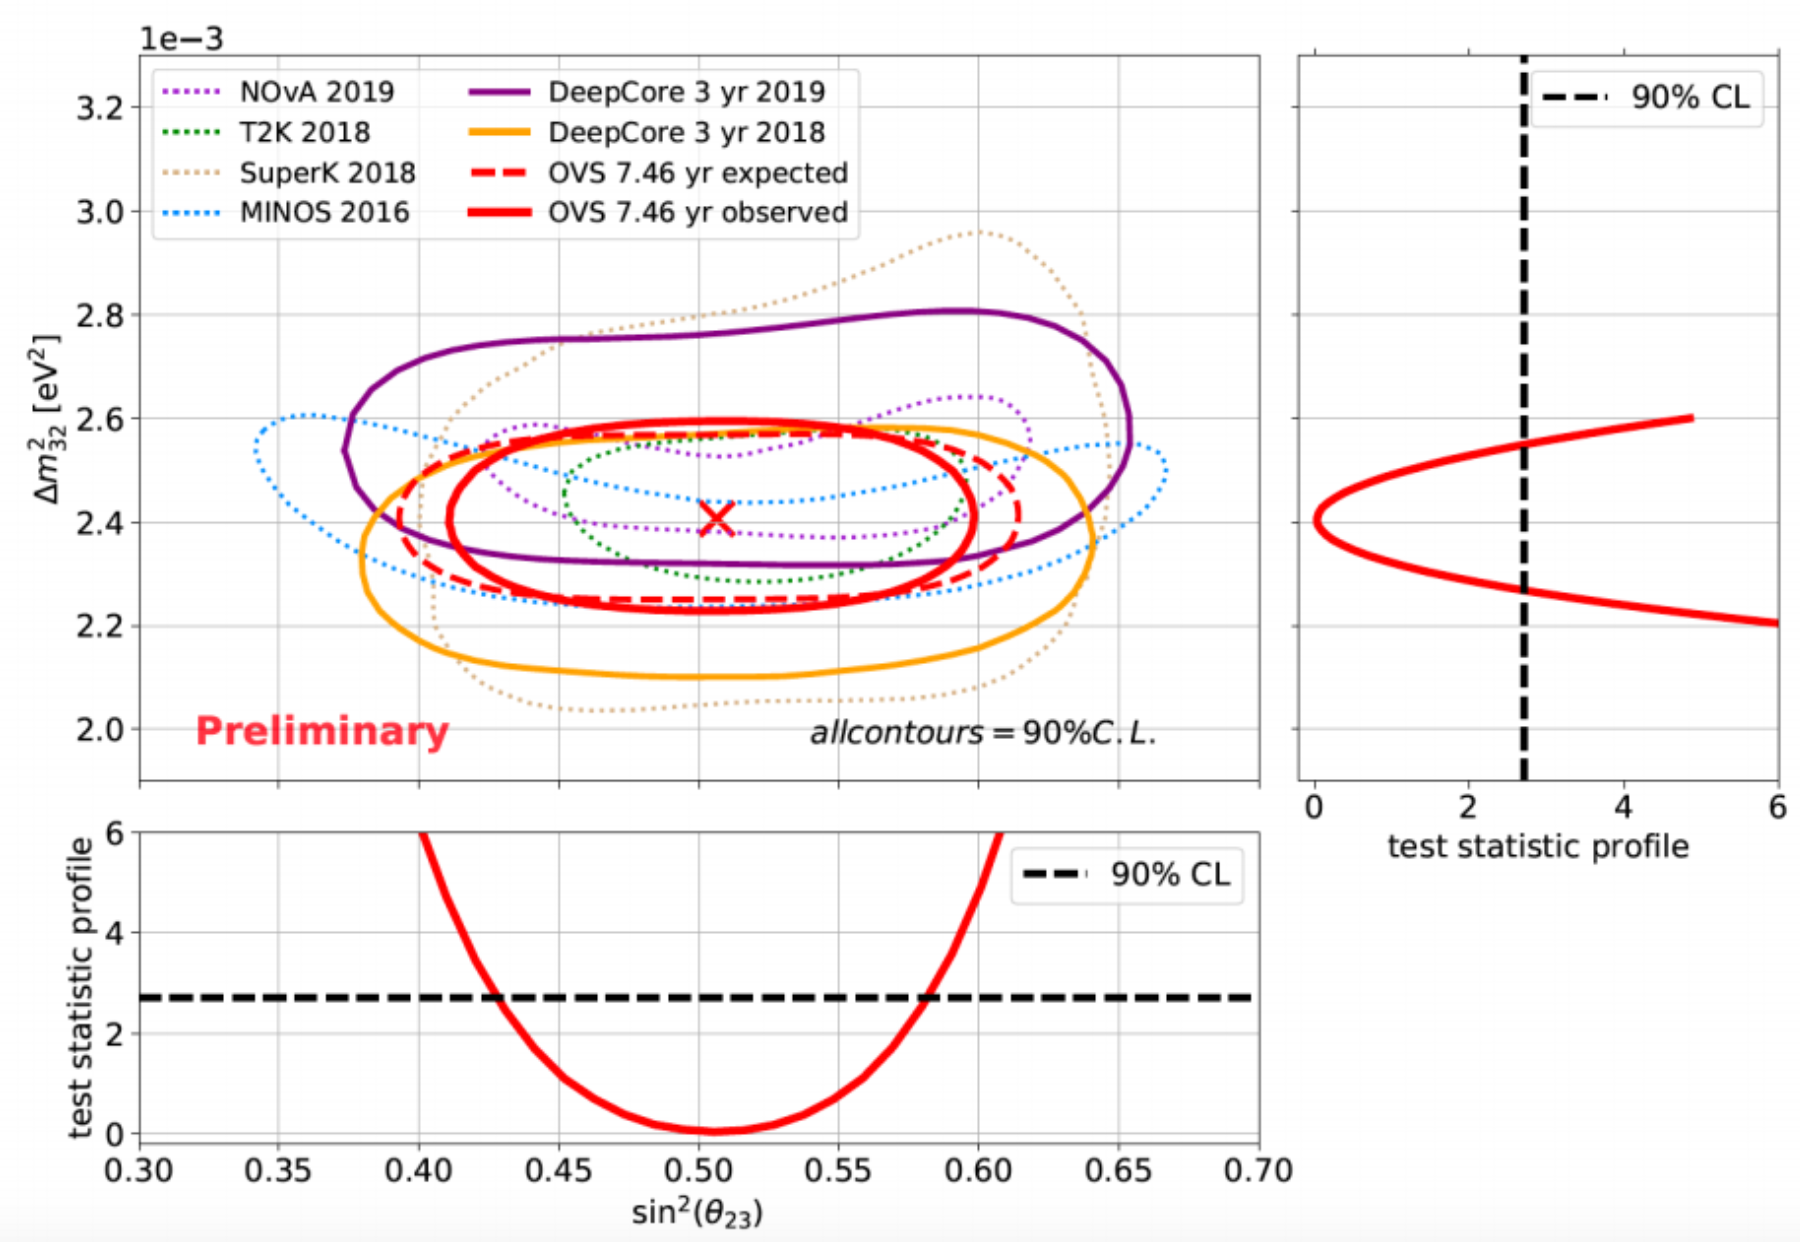
\includegraphics[width=\textwidth]{figures/measurement/three_flavor/results/real_data_contour.png}  
  \tikzsetnextfilename{three_flavor_contour}%
\begin{tikzpicture}

\begin{axis}[
	xmin=0.32, xmax=0.68,
	ymin=1.9e-3, ymax=3.3e-3,
	xmajorgrids, ymajorgrids,
	legend columns=2,
	transpose legend=false,
	xlabel={$\sin^2(\theta_{23})$},
	ylabel={$\Delta m^2_{32}\;(\mathrm{eV^2})$},
	ytick distance=0.2e-3
]

\addplot [orange, thick] table [header=false] {figures/measurement/three_flavor/results/contours/SuperK__sin2_theta23_dm2_32__90pc_2020.csv};
\addlegendentry{SuperK 2020}

\addplot [skyblue, thick, densely dotted] table [header=false] {figures/measurement/three_flavor/results/contours/MINOS_numu_disappearance_90pc_2016.csv};
\addlegendentry{MINOS 2016}

\addplot [bluishgreen, thick, densely dotted] table [header=false] {figures/measurement/three_flavor/results/contours/T2K_sin2_theta23_dm2_32__90pc_2020.csv};
\addlegendentry{T2K 2020}

\addplot [vermilion, thick, densely dotted] table [header=false] {figures/measurement/three_flavor/results/contours/NOvA__sin2_theta23_dm2_32__90pc_2021.csv};
\addlegendentry{NO$\nu$A 2021}

\addplot [black, thick, dashed] table [col sep=comma, header=false] {figures/measurement/three_flavor/results/contours/DeepCore_oscNext_verification_sample__sin2_theta23_dm2_32__90pc_sens_at_bfp_all_syst_bugfix.csv};
\addlegendentry{this work (sensitivity)}

%\addplot [black, thick, dashed] table [col sep=comma, header=false] {figures/measurement/three_flavor/results/contours/DeepCore_oscNext_verification_sample__sin2_theta23_dm2_32__90pc_sens_at_bfp_bugfix.csv};
%\addlegendentry{sensitivity at nominal}

\addplot [black, very thick] table [col sep=comma, header=false] {figures/measurement/three_flavor/results/contours/DeepCore_oscNext_verification_sample__sin2_theta23_dm2_32__90pc_result_bugfix.csv};
\addlegendentry{this work}

% best fit point
\addplot [mark=otimes] coordinates{(0.507, 2.41937e-3)};

\node[plot annotation, text width=3.5 cm, anchor=south west] at (axis description cs:0.01, 0.01) {all contours 90\% C.L.};
% \node[font=\sffamily\footnotesize, red, anchor=south east] at (axis description cs:0.99, 0.01) {\emph{IceCube preliminary}};

\end{axis}

\end{tikzpicture}
  \caption{Contours showing the 90\% C.L. allowed region for the physics parameters of the three-flavor analysis and of other experiments\cite{SK2020,t2k_neutrino_2020,MINOS:2020llm,NOvA:2021nfi}. The sensitivity for this work is calculated at the best fit point and the cross shows the best fit value. Other experiments shown in dotted lines are accelerator results, while solid lines are atmospheric oscillation results. All contours shown assume Normal Ordering.
  \label{fig:real_data_contour_three_flavor}}
\end{figure}

\begin{figure}
    \centering
    %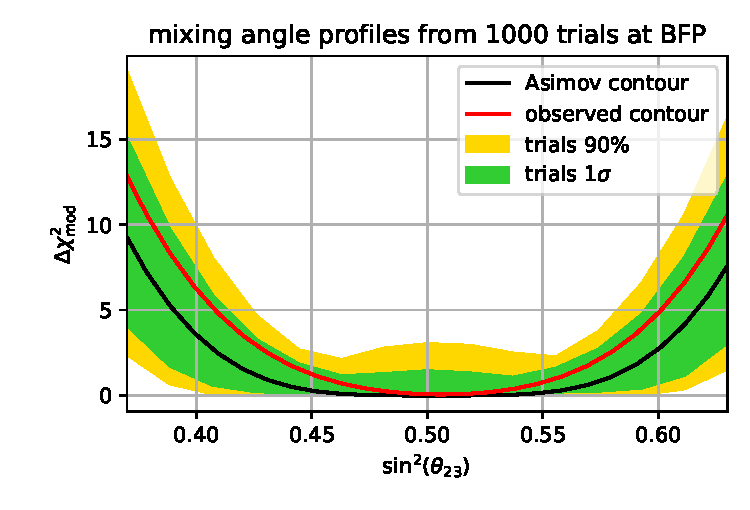
\includegraphics[width=0.8\textwidth]{figures/measurement/three_flavor/results/mixing_brazil_band.pdf}  
    \tikzsetnextfilename{three_flavor_mixing_brazil_band}%
\begin{tikzpicture}
\pgfplotstableread[col sep=comma]{figures/measurement/three_flavor/results/brazil_bands/mixing_brazil_band_data.csv}\table

\pgfplotsset{set layers=axis on top}

% 68% interval: 0.45422922, 0.55732256
% 90% interval: 0.42675708, 0.58344331
% BFP: 0.507

\begin{axis}[
    xmin=0.37, xmax=0.63,
    %xmin=0.32, xmax=0.68,
    ymin=0, ymax=6,
    xmajorgrids,
    %ymajorgrids,
    xlabel={$\sin^2(\theta_{23})$},
    ylabel={$\Delta \chi^2_\mathrm{mod}$},
    ylabel style={at={(-0.1,0.5)}},
    height=0.45\linewidth,
    width=0.8\linewidth,
    % extra x ticks={0.42675708, 0.45422922, 0.55732256, 0.58344331},
    % extra x tick labels={90\% lower, $-1\sigma$, $+1\sigma$, 90\% upper},
    % extra x tick style={grid=major},
    extra y ticks={0.988946481478023, 2.705543454095404},
    extra y tick labels={$1\sigma$, 90\%},
    extra y tick style={grid=major}
    %ytick distance=2
]

\addplot[black, very thick] table [x=sin2_theta23, y=metric_real_data] \table;
\addlegendentry{observed}
\addplot[black, thick, dashed] table [x=sin2_theta23, y=metric_asimov] \table;
\addlegendentry{sensitivity}

%\addplot[blue] table [x=sin2_theta23, y=median_contour] \table;

\addplot[yellow, name path=pct_90_lo, forget plot] table [x=sin2_theta23, y=pct_90_lo] \table;
\addplot[yellow, name path=pct_90_hi, forget plot] table [x=sin2_theta23, y=pct_90_hi] \table;
\addplot[yellow] fill between [of=pct_90_lo and pct_90_hi];
\addlegendentry{90\% band}

\addplot[green, name path=pct_68_lo, forget plot] table [x=sin2_theta23, y=pct_68_lo] \table;
\addplot[green, name path=pct_68_hi, forget plot] table [x=sin2_theta23, y=pct_68_hi] \table;
\addplot[green] fill between [of=pct_68_lo and pct_68_hi];
\addlegendentry{68\% band}

\end{axis}
\end{tikzpicture}

    \caption{Observed contour in $\sin^2(\theta_{23})$ (solid) compared to the Asimov expectation (dashed) and the distribution of 100 pseudo-data trials (yellow and green bands) produced at the best fit point of the three-flavor oscillation analysis. The observed contour is fully contained within 68\% of the fluctuations of the trials.
  \label{fig:mixing_brazil_band_three_flavor}}
\end{figure}

\subsection{Post-fit Data/MC agreement}

Using the weights of the MC events at the best fit point, the post-fit agreement between data and simulation can be shown for any variable. Of particular interest is the distribution of the argument to neutrino oscillations, $L/E$, where $L$ is the total distance traveled by a neutrino and $E$ is its energy. Although the true value of the oscillation argument is unknown for data events, it can nevertheless be calculated from the reconstructed energy and zenith angle. The resulting distribution is shown in \reffig{data_mc_post_fit_l_over_e} and displays a good agreement between data and simulation, with a reduced $\chi^2$ of close to unity. The comparison between data and simulation for the reconstructed zenith angle and energy gives reduced $\chi^2$ values of 0.782 and 1.19, respectively, when calculated in the same binning as is shown in the pre-fit comparison in \reffig{pre-fit-energy-coszen}.

% \begin{figure*}
%     \centering
%     \ref{reco_coszen_postfit_threeflav_legend}\par
%     \tikzsetnextfilename{final_level_postfit_three_flav_reco_coszen}%
\begin{tikzpicture}
    \pgfplotstableread{figures/measurement/three_flavor/results/data_mc_post_fit/reco_coszen.csv}\table
    \begin{groupplot}[
        xmin=-1.055,xmax=0.15500000000000003,
        xmode=normal,
        xmajorgrids, ymajorgrids,
        width=0.45\linewidth,
        ylabel style={at={(-0.15,0.5)}},
        group/.cd,
        group size=1 by 2,
        xticklabels at=edge bottom,
        vertical sep=10pt
        ]
    \nextgroupplot[
        height=0.3\linewidth,
        legend cell align={left},
        legend columns=-1,
        legend to name=reco_coszen_postfit_threeflav_legend,
        ymode=log,
        ymin=3e-8, ymax=3e-5,
        ylabel=rate (Hz),
        % add magic filter to correctly handle empty bins in logarithmic y-axes:
        % If a bin-count is too low or zero, it would cause the line to be
        % interrupted, which creates artefacts and ugliness. Instead, we replace
        % these bin-counts with values that are just below the axis limit.
        % Because of the way pgfplots works, the input is the raw number but the
        % output has to be the log. Weird, I know.
        % y filter/.expression={y < 4.228878698498991e-09 ? ln(4.2288786984989913e-10) : ln(y)}
        y filter/.expression={y < \pgfkeysvalueof{/pgfplots/ymin} ? ln(\pgfkeysvalueof{/pgfplots/ymin}) - 1 : ln(y)}
    ]

    \ploterrorband[muon_color]{muon}{1}
    \addlegendentry{atm. muons}

    \ploterrorband[nue_color]{nuenuebar}{1}
    \addlegendentry{$\nu_e + \bar{\nu}_e$}

    \ploterrorband[numu_color]{numunumubar}{1}
    \addlegendentry{$\nu_\mu + \bar{\nu}_\mu$}

    \ploterrorband[nutau_color]{nutaunutaubar}{1}
    \addlegendentry{$\nu_\tau + \bar{\nu}_\tau$}


    % alternative event breakdown by interaction
    % \ploterrorband[nue_color]{nue_ccnuebar_cc}{1}
    % \addlegendentry{$\nu_e + \bar{\nu}_e$, CC}
    %
    % \ploterrorband[numu_color]{numu_ccnumubar_cc}{1}
    % \addlegendentry{$\nu_\mu + \bar{\nu}_\mu$, CC}
    %
    % \ploterrorband[nutau_color]{nutau_ccnutaubar_cc}{1}
    % \addlegendentry{$\nu_\tau + \bar{\nu}_\tau$, CC}
    %
    % \ploterrorband[nc_color]{nuall_ncnuallbar_nc}{1}
    % \addlegendentry{all $\nu$, NC}

    \ploterrorband{total_mc}{1}
    \addlegendentry{total MC}

    \ploterrorbar{data}
    \addlegendentry{data}


    \nextgroupplot[
        height=0.2\linewidth,
        ymin=0.7, ymax=1.3,
        ylabel=rate/total MC,
        xlabel=reconstructed $\cos(\theta_{\mathrm{zenith}})$
    ]

    \ploterrorbar{data_mc_ratio}
    % \plotratioerrorband[muon_color]{muon}{total_mc}
    % \plotratioerrorband[nue_color]{nuenuebar}{total_mc}
    % \plotratioerrorband[numu_color]{numunumubar}{total_mc}
    % \plotratioerrorband[nutau_color]{nutaunutaubar}{total_mc}

    \node[anchor=south, font=\footnotesize] at (axis description cs:0.5, 0.01) {$\chi^2_{\mathrm{mod}}/\mathrm{dof} = 0.782$};
    \end{groupplot}
\end{tikzpicture}

%     \tikzsetnextfilename{final_level_postfit_three_flav_reco_energy}%
\begin{tikzpicture}
    \pgfplotstableread{figures/measurement/three_flavor/results/data_mc_post_fit/reco_energy.csv}\table
    \begin{groupplot}[
        xmin=5.362591587787688,xmax=185.61920737481475,
        xmode=log,
        xmajorgrids, ymajorgrids,
        width=0.45\linewidth,
        ylabel style={at={(-0.15,0.5)}},
        group/.cd,
        group size=1 by 2,
        xticklabels at=edge bottom,
        vertical sep=10pt
        ]
    \nextgroupplot[
        height=0.3\linewidth,
        legend cell align={left},
        legend columns=3,
        legend to name=reco_energy_postfit_threeflav_legend,
        ymode=log,
        ymin=3e-8, ymax=3e-5,
        ylabel=rate (Hz),
        % add magic filter to correctly handle empty bins in logarithmic y-axes:
        % If a bin-count is too low or zero, it would cause the line to be
        % interrupted, which creates artefacts and ugliness. Instead, we replace
        % these bin-counts with values that are just below the axis limit.
        % Because of the way pgfplots works, the input is the raw number but the
        % output has to be the log. Weird, I know.
        % y filter/.expression={y < 1.129498430227963e-09 ? ln(1.1294984302279631e-10) : ln(y)}
        y filter/.expression={y < \pgfkeysvalueof{/pgfplots/ymin} ? ln(\pgfkeysvalueof{/pgfplots/ymin}) - 1 : ln(y)}
    ]

    \ploterrorband[muon_color]{muon}{1}
    \addlegendentry{atm. muons}

    \ploterrorband[nue_color]{nuenuebar}{1}
    \addlegendentry{$\nu_e + \bar{\nu}_e$}

    \ploterrorband[numu_color]{numunumubar}{1}
    \addlegendentry{$\nu_\mu + \bar{\nu}_\mu$}

    \ploterrorband[nutau_color]{nutaunutaubar}{1}
    \addlegendentry{$\nu_\tau + \bar{\nu}_\tau$}


    % alternative event breakdown by interaction
    % \ploterrorband[nue_color]{nue_ccnuebar_cc}{1}
    % \addlegendentry{$\nu_e + \bar{\nu}_e$, CC}
    %
    % \ploterrorband[numu_color]{numu_ccnumubar_cc}{1}
    % \addlegendentry{$\nu_\mu + \bar{\nu}_\mu$, CC}
    %
    % \ploterrorband[nutau_color]{nutau_ccnutaubar_cc}{1}
    % \addlegendentry{$\nu_\tau + \bar{\nu}_\tau$, CC}
    %
    % \ploterrorband[nc_color]{nuall_ncnuallbar_nc}{1}
    % \addlegendentry{all $\nu$, NC}

    \ploterrorband{total_mc}{1}
    \addlegendentry{total MC}

    \ploterrorbar{data}
    \addlegendentry{data}


    \nextgroupplot[
        height=0.2\linewidth,
        ymin=0.7, ymax=1.3,
        ylabel=rate/total MC,
        xlabel=reconstructed energy (GeV)
    ]

    \ploterrorbar{data_mc_ratio}
    % \plotratioerrorband[muon_color]{muon}{total_mc}
    % \plotratioerrorband[nue_color]{nuenuebar}{total_mc}
    % \plotratioerrorband[numu_color]{numunumubar}{total_mc}
    % \plotratioerrorband[nutau_color]{nutaunutaubar}{total_mc}

    \node[anchor=south, font=\footnotesize] at (axis description cs:0.5, 0.01) {$\chi^2_{\mathrm{mod}}/\mathrm{dof} = 1.19$};
    \end{groupplot}
\end{tikzpicture}

%     \caption{Distributions of reconstructed energy and zenith angle at the best fit point of the three-flavor analysis.}
%     \label{fig:post-fit-threeflav-energy-coszen}
% \end{figure*}

\begin{figure}
    \centering
    \tikzsetnextfilename{final_level_postfit_three_flav_l_over_e}%
\begin{tikzpicture}
    \pgfplotstableread{figures/measurement/three_flavor/results/data_mc_post_fit/l_over_e.csv}\table
    \begin{groupplot}[
        xmin=7.6727049901092546,xmax=2606.642641126127,
        xmode=log,
        xmajorgrids, ymajorgrids,
        width=0.8\linewidth,
        ylabel style={at={(-0.15,0.5)}},
        group/.cd,
        group size=1 by 2,
        xticklabels at=edge bottom,
        vertical sep=10pt
        ]
    \nextgroupplot[
        height=0.5\linewidth,
        legend cell align={left},
        legend columns=3,
        ymode=log,
        ymin=3e-8, ymax=8e-5,
        ylabel=rate (Hz),
        % add magic filter to correctly handle empty bins in logarithmic y-axes:
        % If a bin-count is too low or zero, it would cause the line to be
        % interrupted, which creates artefacts and ugliness. Instead, we replace
        % these bin-counts with values that are just below the axis limit.
        % Because of the way pgfplots works, the input is the raw number but the
        % output has to be the log. Weird, I know.
        y filter/.expression={y < \pgfkeysvalueof{/pgfplots/ymin} ? ln(\pgfkeysvalueof{/pgfplots/ymin}) - 1 : ln(y)}
    ]

    \ploterrorband[muon_color]{muon}{1}
    \addlegendentry{atm. muons}

    \ploterrorband[nue_color]{nuenuebar}{1}
    \addlegendentry{$\nu_e + \bar{\nu}_e$}

    \ploterrorband[numu_color]{numunumubar}{1}
    \addlegendentry{$\nu_\mu + \bar{\nu}_\mu$}

    \ploterrorband[nutau_color]{nutaunutaubar}{1}
    \addlegendentry{$\nu_\tau + \bar{\nu}_\tau$}


    % alternative event breakdown by interaction
    % \ploterrorband[nue_color]{nue_ccnuebar_cc}{1}
    % \addlegendentry{$\nu_e + \bar{\nu}_e$, CC}
    %
    % \ploterrorband[numu_color]{numu_ccnumubar_cc}{1}
    % \addlegendentry{$\nu_\mu + \bar{\nu}_\mu$, CC}
    %
    % \ploterrorband[nutau_color]{nutau_ccnutaubar_cc}{1}
    % \addlegendentry{$\nu_\tau + \bar{\nu}_\tau$, CC}
    %
    % \ploterrorband[nc_color]{nuall_ncnuallbar_nc}{1}
    % \addlegendentry{all $\nu$, NC}

    \ploterrorband{total_mc}{1}
    \addlegendentry{total MC}

    \ploterrorbar{data}
    \addlegendentry{data}


    \nextgroupplot[
        height=0.30\linewidth,
        ymin=0.7, ymax=1.3,
        ylabel=rate/total MC,
        xlabel=L/E (km/GeV)
    ]

    \ploterrorbar{data_mc_ratio}
    % \plotratioerrorband[muon_color]{muon}{total_mc}
    % \plotratioerrorband[nue_color]{nuenuebar}{total_mc}
    % \plotratioerrorband[numu_color]{numunumubar}{total_mc}
    % \plotratioerrorband[nutau_color]{nutaunutaubar}{total_mc}

    \node[anchor=south, font=\footnotesize] at (axis description cs:0.5, 0.01) {$\chi^2_{\mathrm{mod}}/\mathrm{dof} = 0.986$};
    \end{groupplot}
\end{tikzpicture}

    \caption{Oscillation argument $L/E$ calculated from reconstructed quantities at the best fit point of the three-flavor oscillation analysis.}
    \label{fig:data_mc_post_fit_l_over_e}
\end{figure}
